%!TEX TS-program = pdflatex
%!TEX TS-program = skim
%
%  PyMC User's Guide
%
%  Created by Chris Fonnesbeck on 2006-05-03.
%  Copyright (c) 2006 . All rights reserved.
%
\documentclass[article]{jss}

%% almost as usual
\author{Anand Patil}
\title{A Gaussian process module for \pkg{PyMC}}

%% for pretty printing and a nice hypersummary also set:
\Plainauthor{Anand Patil} %% comma-separated
\Plaintitle{A Gaussian process module for PyMC} %% without formatting
% \Shorttitle{GP's For PyMC} %% a short title (if necessary)

%% an abstract and keywords
\Abstract{
  This article introduces a package adding Gaussian process functionality to the Bayesian analysis package \pkg{PyMC}. Gaussian processes (GPs) are probability distributions for functions. In Bayesian statistics, they are often used as priors for functions whose forms are unknown. They can encode many types of knowledge about functions, yet remain much less restrictive than priors based on particular functional forms. GPs are not hard to understand at a conceptual level, but implementing them efficiently on a computer can require fairly involved linear algebra. This package implements Gaussian processes as a set of \proglang{Python} classes that can support many types of usage, from intuitive exploration to embedding them in larger probability models and fitting with MCMC.
}
\Keywords{gassian process, bayesian, \proglang{Python}}
\Plainkeywords{gaussian process, bayesian, Python} %% without formatting
%% at least one keyword must be supplied

%% publication information
%% NOTE: Typically, this can be left commented and will be filled out by the technical editor
%% \Volume{13}
%% \Issue{9}
%% \Month{September}
%% \Year{2004}
%% \Submitdate{2004-09-29}
%% \Acceptdate{2004-09-29}

%% The address of (at least) one author should be given
%% in the following format:
\Address{
  Anand Patil\\
  Malaria Atlas Project\\
  Department of Zoology\\
  University of Oxford\\
  Oxford, OX1 3PS, UK\\
  E-mail: \email{anand.patil@zoo.ox.ac.uk}
}

% Use utf-8 encoding for foreign characters
%\usepackage[utf8]{inputenc}

% % Setup for fullpage use
% \usepackage{fullpage}
% \usepackage{amsmath}
\usepackage{epsfig}
\usepackage{upquote} 
\usepackage{verbatim} 
% 
% % \usepackage{pdfsync}
% 
% % Flexible citation syntax
% \usepackage{natbib}
% % Uncomment some of the following if you use the features
% %
% 
% % Multipart figures
% %\usepackage{subfigure}
% 
% % More symbols
% \usepackage{amsmath}
% \usepackage{amssymb}
% % \usepackage{latexsym}
% 
% % Package for including code in the document
% \usepackage{listings}
% 
% % Surround parts of graphics with box
% %\usepackage{boxedminipage}
% 
% % This is now the recommended way for checking for PDFLaTeX:
% \usepackage{ifpdf}
% 
% % Enable hyperlinks
% % \usepackage[pdfpagemode=FullScreen,colorlinks=true,linkcolor=red]{hyperref}
% 
% % \ifpdf
% % \usepackage[pdftex]{graphicx}
% % \else
% % \usepackage{graphicx}
% % \fi
% 
% %%% EPYDOC STUFF %%%
\usepackage{underscore}

\begin{document}

\maketitle

\tableofcontents


\section{Introduction}\label{sec:firstlook}

Gaussian processes are probability distributions for mathematical functions. The statement `random function $f$ has a Gaussian process distribution with mean $M$ and covariance $C$' is usually written as follows:
\begin{equation}
    f\sim\textup{GP}(M,C).
\end{equation}
The two parameters of the distribution are analogous to the parameters of the normal distribution. $M$ is the mean function, $M(x)=\E(f(x))$. $C$ is the covariance function, $C(x,y)=\COV(f(x),f(y))$. Among other things, $C$ regulates the amount by which $f$ may deviate from $M$ at any input value $x$, the roughnesss of $f$ and the typical lengthscale of changes in $f$.

As with any probability distribution, random values can be drawn from a Gaussian process. However, these values (called `realizations') are actually mathematical functions rather than the usual numbers or vectors. This package represents these random values as \code{Realization} objects which, in accordance with intuition, behave like \proglang{Python} functions with a few extra features.

Gaussian processes, represented by \pkg{PyMC} stochastic variables \citep{pymc} valued as \code{Realization} objects, can be embedded in larger probability models. These models can be fit using Markov chain Monte Carlo \cite{gamerman}, after which the `dynamic trace' for each Gaussian process consists of a list, array or on-disk database containing \code{Realization} objects sampled from the target distribution. This intuitive object model simplifies and expedites construction and fitting of probability models, as well as predictive simulation.

To improve performance, all of this package's numerical computations are done in C or Fortran extensions, some of which are provided by the \pkg{NumPy} package \citep{numpybook}. Covariance function evaluations are multithreaded for sufficiently large matrices.

All examples can be found in the folder \code{pymc/examples/gp} in the \pkg{PyMC} source tree. 

\section{Creating a Gaussian process}\label{sub:inst}

This section demonstrates creation of a covariance function, a mean function, and finally several random functions drawn from the Gaussian process distribution defined by those objects.

\subsection{Creating a mean function}\label{subsub:mean}

\begin{figure}
    \centering
        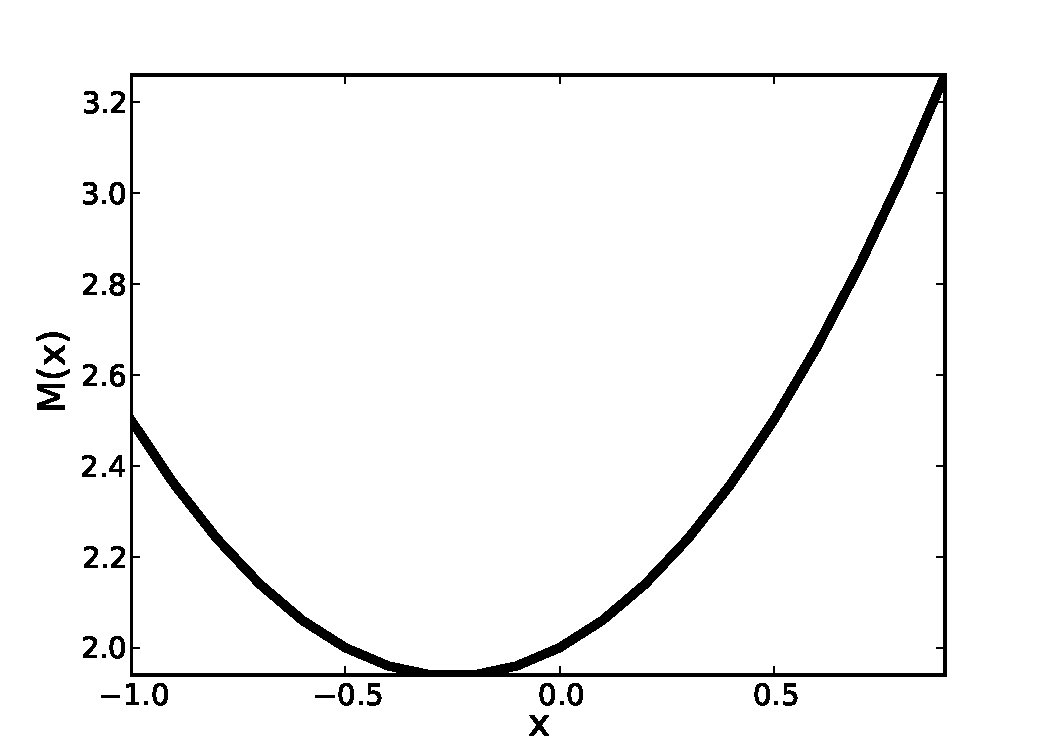
\epsfig{file=figs/mean.pdf,width=8cm}
    \caption{The mean function generated by {\sffamily `examples/mean.py'}.}
    \label{fig:mean}
\end{figure}

The mean function of a univariate Gaussian process can be interpreted as a prior guess for the GP, so it is also a univariate function. Mean functions are represented by class \code{Mean}, which is a wrapper for an ordinary \proglang{Python} function. We will use the parabolic function
\begin{equation}
    M(x) = ax^2 + bx + c.
\end{equation}

The following code (from \code{pymc/examples/gp/Mean.py}) will produce an instance of class \code{Mean} called $M$:
\begin{CodeChunk}
\begin{CodeInput}
from pymc.gp import *
def quadfun(x, a, b, c):
    return (a * x ** 2 + b * x + c)
M = Mean(quadfun, a = 1., b = .5, c = 2.)        
\end{CodeInput}
\end{CodeChunk}

The first argument of \code{Mean}'s init method is the underlying \proglang{Python} function, in this case \code{quadfun}. The extra arguments $a$, $b$  and $c$ will be memorized and passed to \code{quadfun} whenever $M$ is called; the call $M(x)$ in the plotting portion of the script does not need to pass them in.

Mean functions broadcast over their arguments in the same way as \href{http://docs.scipy.org/doc/numpy/reference/ufuncs.html}{\pkg{NumPy} universal functions} \citep{numpybook}, which means that the call $M(x)$, where $x$ is a vector, returns the vector
\begin{eqnarray*}
    [M(x_0),\ldots, M(x_{N-1})].
\end{eqnarray*}

The last part of the code plots $M(x)$ on $-1<x<1$, and its output is shown in figure \ref{fig:mean}. As expected, the plot is a parabola.

\subsection{Creating a covariance function}\label{subsub:cov}
\begin{figure}
    \centering
        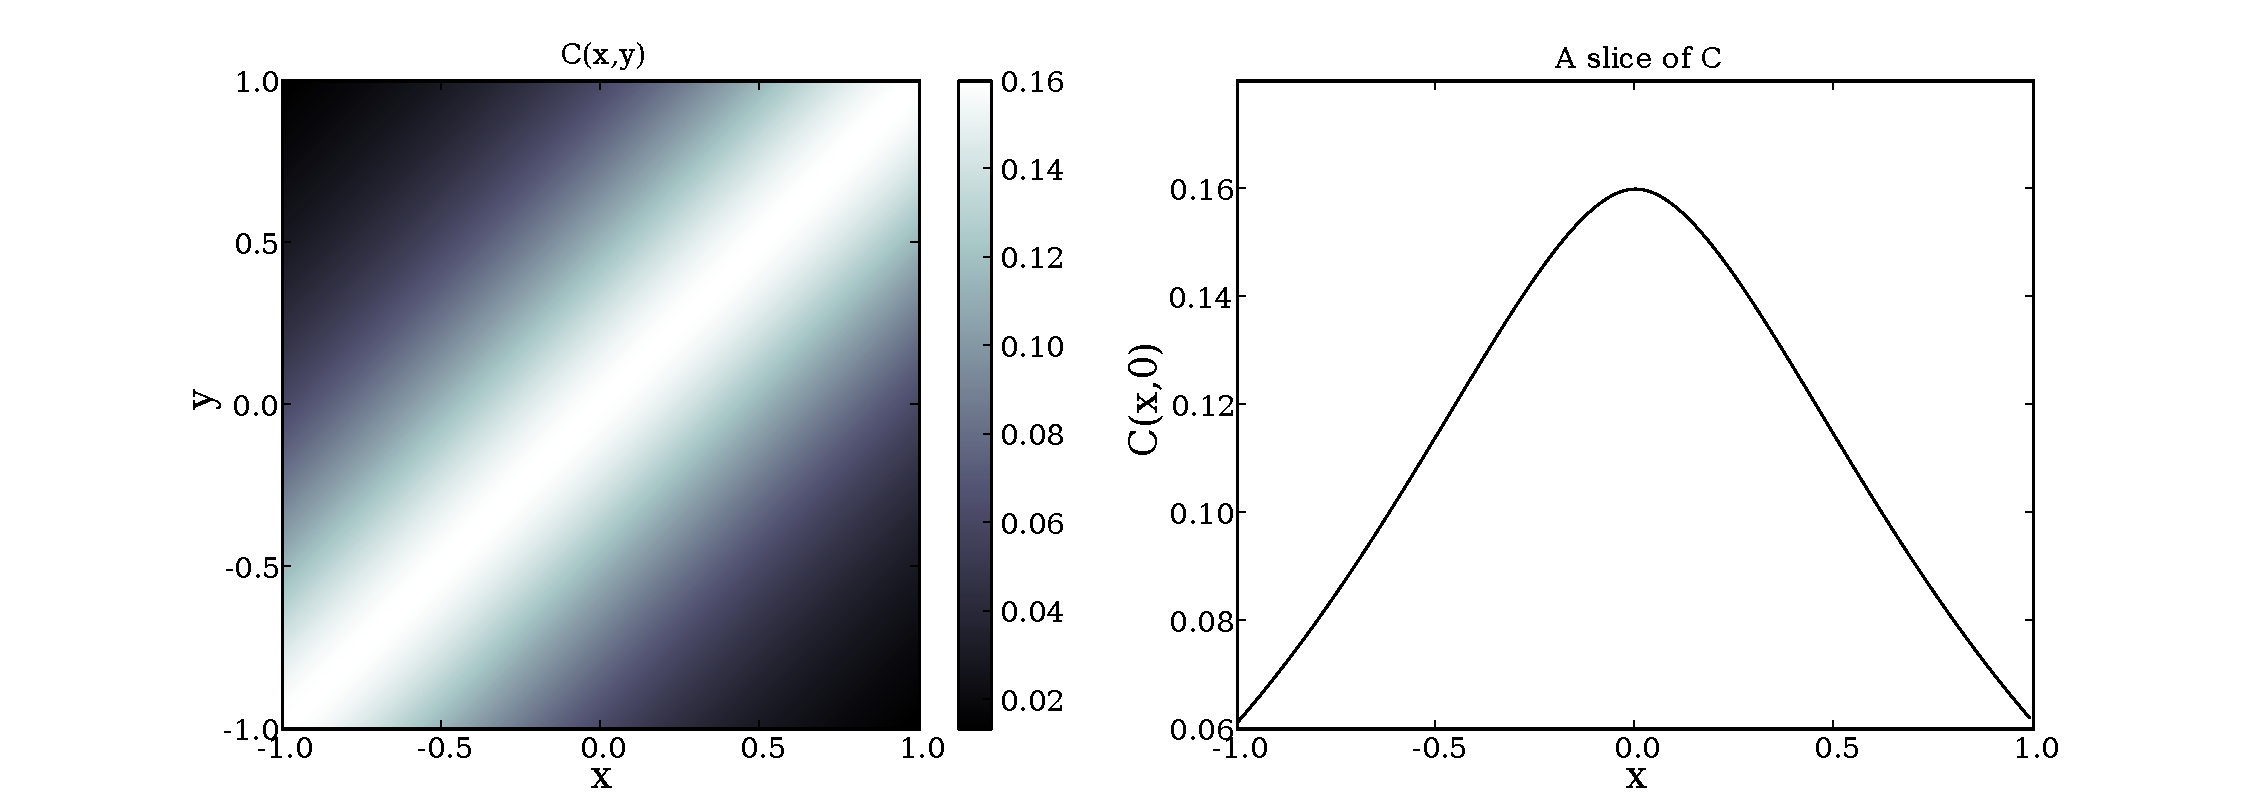
\epsfig{file=figs/cov.pdf,width=12cm}
    \caption{The covariance function generated by {\sffamily `examples/cov.py'}. On the left is the covariance function $C(x,y)$ evaluated over a square: $-1\le x\le 1,\ -1\le y\le 1$. On the right is a slice of the covariance: $C(x,0)$ for $0\le x \le 1$}
    \label{fig:cov}
\end{figure}

Gaussian process covariance functions are represented by the class \code{Covariance}, which like \code{Mean} is essentially a wrapper for ordinary \proglang{Python} functions. The example in \code{pymc/examples/gp/cov.py} uses the popular Mat\`ern covariance function \citep{banerjee}, which is provided in module \code{cov_funs}. In addition to the two arguments $x$ and $y$, the Mat\`ern covariance function takes three parameters: \code{amp} controls the amount by which realizations may deviate from their mean, \code{diff_degree} controls the roughness of realizations (the degree of differentiability), and \code{scale} controls the lengthscale over which realizations change.

The user is free to write functions to wrap in \code{Covariance} objects. See \href{http://code.google.com/p/pymc}{the package documentation} for more information.

The code in \code{pymc/examples/gp/cov.py} will produce an instance of class \code{Covariance} called $C$:
\begin{CodeChunk}
\begin{CodeInput}
from pymc.gp import *
from pymc.gp.cov_funs import matern

C = Covariance(eval_fun = matern.euclidean, diff_degree = 1.4, amp = .4, scale = 1.)
\end{CodeInput}
\end{CodeChunk}

The first argument to \code{Covariance}'s init method is the \proglang{Python} function from which the covariance function will be made. In this case, \code{eval_fun} is \code{matern.euclidean}. Covariance functions' calling conventions are slightly different from ordinary \pkg{NumPy} universal functions' \citep{numpybook} in two ways. First, broadcasting works differently. If $C$ were a \pkg{NumPy} universal function, $C(x,y)$ would return the following array:
    \begin{eqnarray*}
        \begin{array}{ccc}
            [C(x_0,y_0)& \ldots& C(x_{N-1},y_{N-1})],
        \end{array}
    \end{eqnarray*}
    where $x$ and $y$ would need to be vectors of the same length. In fact $C(x,y)$ returns a matrix:
    \begin{eqnarray*}
        \left[\begin{array}{ccc}
            C(x_0,y_0)& \ldots& C(x_0,y_{N_y-1})\\
            \vdots&\ddots&\vdots\\
            C(x_{N_x-1},y_0)& \ldots& C(x_{N_x-1},y_{N_y-1})
        \end{array}\right],
    \end{eqnarray*}
    and input arguments $x$ and $y$ don't need to be the same length. Second, covariance functions can be called with just one argument. $C(x)$ returns
    \begin{eqnarray*}
         [C(x_0,x_0)& \ldots& C(x_{N_x-1},x_{N_x-1})] = \textup{diag}(C(x,x)),
    \end{eqnarray*}
    but is computed much faster than diag$(C(x,x))$ would be.
The extra arguments \code{diff_degree, amp} and \code{scale}, which are required by \code{matern.euclidean}, will be passed to \code{matern.euclidean} by $C$ every time is called.
 
The output of \code{examples/cov.py} is shown in figure \ref{fig:cov}.

\subsubsection{Cholesky algorithms}

The numerical `heavy lifting' done by this package is primarily handled by \code{Covariance} and its subclasses. \texttt{Covariance} itself bases all its computations on the incomplete Cholesky decomposition algorithm used by the \proglang{Matlap} package \pkg{chol_incomplete} \citep{seeger}. \code{Covariance} computes rows of covariance matrices as they are needed, so if the function it wraps tends to produce covariance matrices with only a few large eigenvalues it can compute the Cholesky decomposition in less than $O(n^2)$ arithmetic operations \citep{predictivechol}.

\code{Covariance} calls back to \proglang{Python} from \proglang{Fortran} every time it needs a new row. If the function it wraps tends to produce full-rank covariance matrices (for which all rows are required), this is inefficient. \code{FullRankCovariance} is a drop-in replacement for \code{Covariance} that is much faster, but fails (with a helpful error message) if it attempts to factor a matrix that is not full rank. \code{NearlyFullRankCovariance} provides a compromise between the two: it computes covariance matrices in full in \proglang{Fortran}, then factors them using the robust algorithm of \pkg{chol_incomplete}.

\subsection{Drawing realizations}\label{subsub:realizations}
\begin{figure}
    \centering
        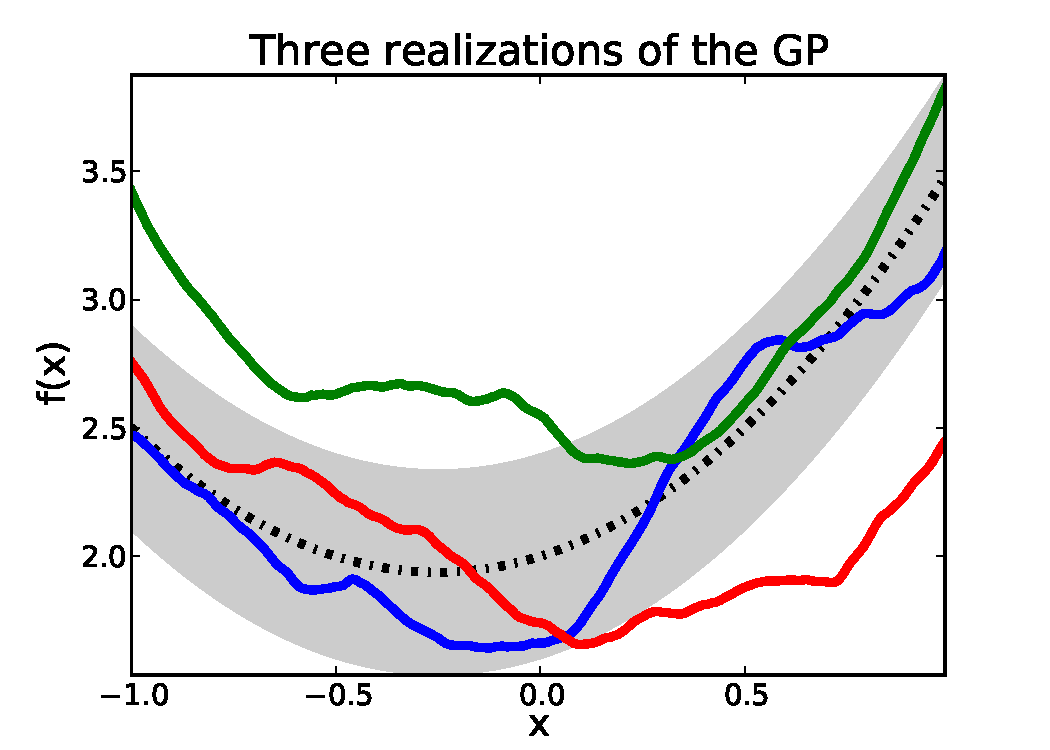
\epsfig{file=figs/realizations.pdf,width=8cm}
    \caption{Three realizations from a Gaussian process displayed with mean $\pm$ 1 sd envelope. Generated by {\sffamily `examples/realizations.py'}.}
    \label{fig:realizations}
\end{figure}

The code in \texttt{pymc/examples/gp/realizations.py} generates a list of \code{Realization} objects, which represent realizations (draws) from the Gaussian process defined by $M$ and $C$:
\begin{CodeChunk}
\begin{CodeInput}
from mean import M
from cov import C
from pymc.gp import *

f_list = [Realization(M,C) for i in range(3)]
\end{CodeInput}
\end{CodeChunk}

The init method of \code{Realization} takes only two required arguments, a \code{Mean} object and a \code{Covariance} object. Each element of \code{f_list} is a Gaussian process realization, which is essentially a randomly-generated \proglang{Python} function. Like \code{Mean} objects, \code{Realization} objects use the same broadcasting rules as \pkg{NumPy} universal functions. The call $f(x)$ returns the vector
\begin{eqnarray*}
    [f(x_0)\ldots f(x_{N-1})].
\end{eqnarray*}

Each of the three realizations in \code{f_list} is plotted in figure \ref{fig:realizations}, superimposed on a $\pm$ 1 standard deviation envelope.


\section{Nonparametric regression: observing Gaussian processes}\label{sec:observing}

\begin{figure}
    \centering
        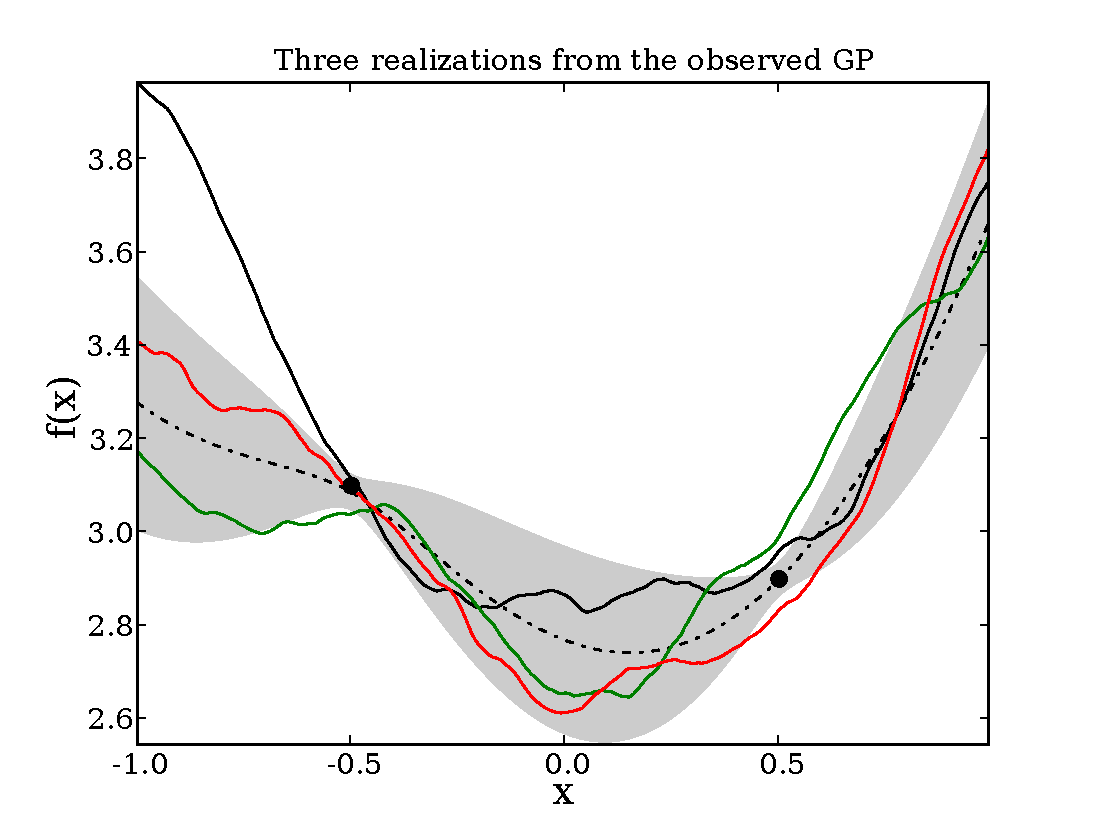
\epsfig{file=figs/obs.pdf,width=5cm}
        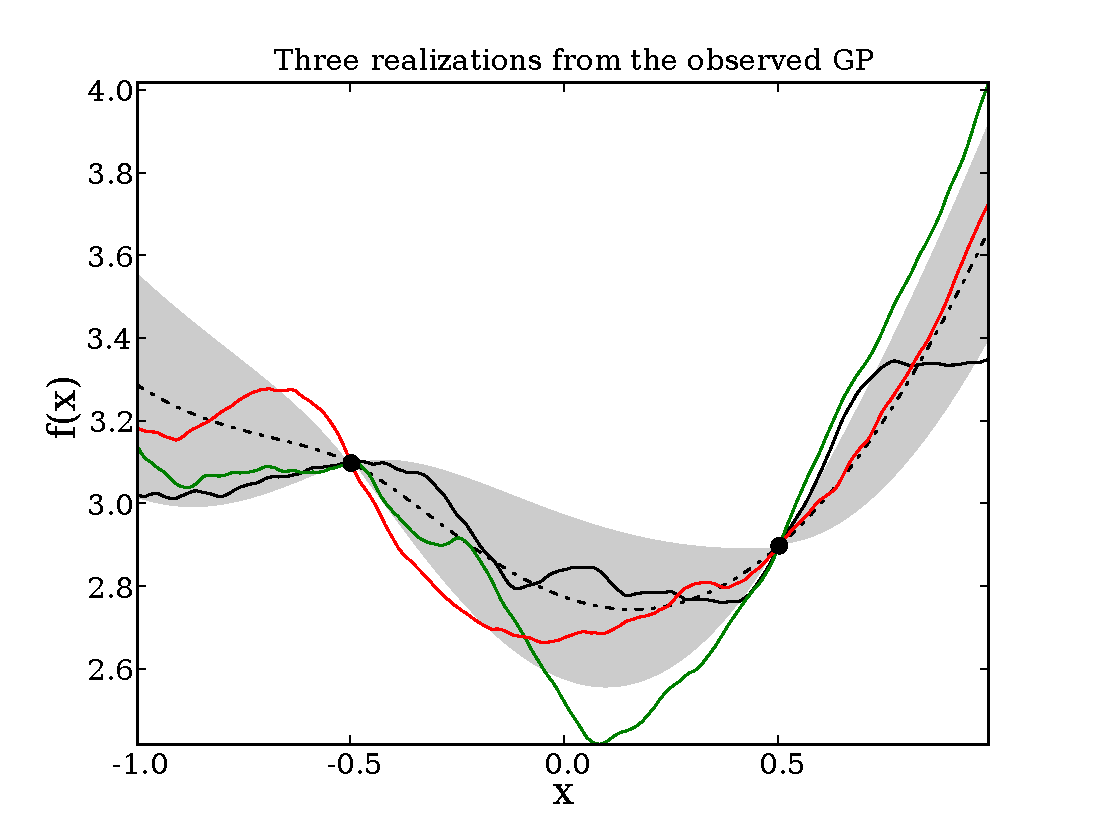
\epsfig{file=figs/cond.pdf,width=5cm}
    \caption{The output of {\sffamily `examples/observations.py'}: the observed GP with \code{obs_V = .002} (left) and \code{obs_V = 0} (right). Note that in the conditioned case, the $\pm$ 1 SD envelope shrinks to zero at the points where the observations were made, and all realizations pass through the observed values. Compare these plots to those in figure \ref{fig:realizations}.}
    \label{fig:obs}
\end{figure}

Consider the following common statistical situation: A Gaussian process prior for an unknown function $f$ is chosen, then the value of $f$ is observed at $N$ input points $[o_0\ldots o_{N-1}]$, possibly with uncertainty. If the observation error is normally distributed, it turns out that $f$'s posterior distribution given the new information is another Gaussian process, with new mean and covariance functions.

The probability model that represents this situation is as follows:
\begin{equation}
    \label{regprior}
    \left.\begin{array}{l}
        \textup{data}_i \stackrel{\tiny{\textup{ind}}}{\sim} \textup{N}(f(o_i), V_i)\\
        f \sim \textup{GP}(M,C)\\
    \end{array}\right\}\Rightarrow f|\textup{data} \sim \textup{GP}(M_o, C_o).
\end{equation}
Function \code{observe} imposes normally-distributed observations on Gaussian process distributions. This function converts $f$'s prior to its posterior by transforming $M$ and $C$ in equation \ref{regprior} to $M_o$ and $C_o$:

The code in \code{pymc/examples/gp/observation.py} imposes the observations
\begin{eqnarray*}
    f(-.5) = 3.1\\
    f(.5) = 2.9
\end{eqnarray*}
with observation variance $V=.002$ on the GP distribution defined in \code{mean.py} and \code{cov.py}:
\begin{CodeChunk}
\begin{CodeInput}
from mean import M
from cov import C
from pymc.gp import *
from numpy import *

obs_x = array([-.5,.5])
V = array([.002,.002])
data = array([3.1, 2.9])
observe(M=M, C=C, obs_mesh=obs_x, obs_V=V, obs_vals=data)

f_list = [Realization(M,C) for i in range(3)]
\end{CodeInput}
\end{CodeChunk}

The function \code{observe} takes a covariance $C$ and a mean $M$ as arguments, and essentially tells them that their realizations' values on \code{obs_mesh} have been observed to be \code{obs_vals} with variance \code{obs_V}. If \code{obs_V} is \code{None}, \code{observe} assumes that the observation variance was zero.

The output of \code{observation.py}  is shown in figure \ref{fig:obs}, along with the output with \code{obs_V=None}. Compare these to the analogous figure for the unobserved GP, figure \ref{fig:realizations}. The covariance after observation is visualized in figure \ref{fig:obscov}. The covariance `tent' has been pressed down at points where $x\approx \pm .5$ and/or $y\approx\pm .5$, which are the values where the observations were made.

\begin{figure}
    \centering
        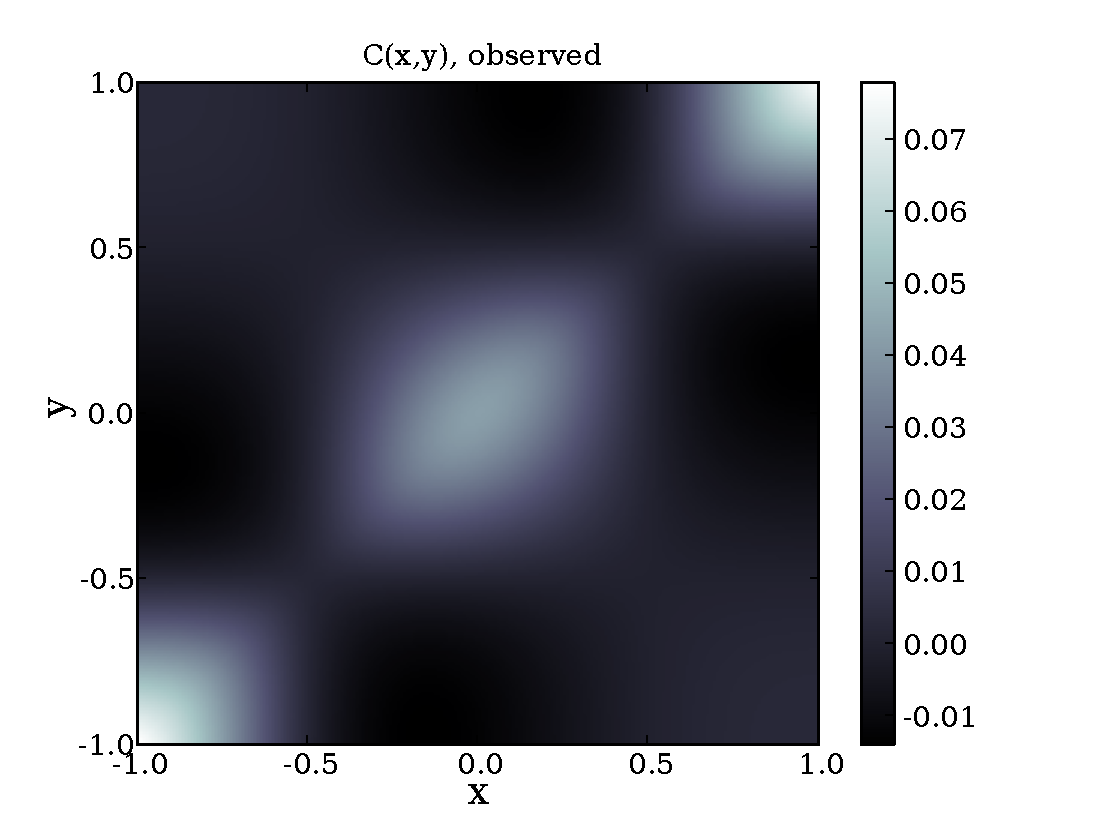
\epsfig{file=figs/obscov.pdf,width=5cm}
    \caption{The covariance function from {\sffamily `observation.py'} after observation. Compare this with the covariance function before observation, visualized in figure \ref{fig:cov} }
    \label{fig:obscov}
\end{figure}

\section{Higher-dimensional GPs}\label{sec:highdim}

In addition to functions of one variable such as $f(x)$, this package supports Gaussian process priors for functions of many variables such as $f(\mathbf{x})$, where $\mathbf{x}=[x_0\ldots x_{n-1}]$. This is useful for modeling dynamical or biological functions of many variables as well as for spatial statistics.

When array is passed into a \code{Mean}, \code{Covariance} or \code{Realization}'s init method or one of these objects is evaluated on an array, the convention is that the array's last index iterates over spatial dimension. To evaluate a covariance $C$ on the ordered pairs $(0,1)$, $(2,3)$, $(4,5)$ and $(6,7)$, the user could pass in the following two-dimensional \pkg{NumPy} array:
\begin{verbatim}
[[0,1]
 [2,3]
 [4,5]
 [6,7]]
\end{verbatim}
or the following three-dimensional array:
\begin{verbatim}
[[[0,1]
  [2,3]],

  [4,5]
  [6,7]]]
\end{verbatim}
Either is fine, since in both the last index iterates over elements of the ordered pairs.

The exception to this rule is one-dimensional input arrays. The array
\begin{verbatim}
[0, 1, 2, 3, 4, 5, 6, 7]
\end{verbatim}
is interpreted as an array of eight one-dimensional values, whereas the array
\begin{verbatim}
[[0, 1, 2, 3, 4, 5, 6, 7]]
\end{verbatim}
is interpreted as a single eight-dimensional value according to the convention above.

Means and covariances learn their spatial dimension the first time they are called or observed. Some covariances, such as those specified in geographic coordinates, have an intrinsic spatial dimension. Realizations inherit their spatial dimension from their means and covariances when possible, otherwise they infer it the first time they are called. If one of these objects is subsequently called with an input of a different dimension, it raises an error.

\subsection{Covariance function bundles and coordinate systems}
The examples so far, starting with \code{examples/cov.py}, have used the covariance function \code{matern.euclidean}. This function is an attribute of the \code{matern} object, which is an instance of class \code{covariance_function_bundle}.

Instances of \code{covariance_function_bundle} have three attributes, \code{euclidean}, \code{geo_deg} and \code{geo_rad}, which correspond to standard coordinate systems:
\begin{itemize}
    \item \code{euclidean}: $n$-dimensional Euclidean coordinates.
    \item \code{geo_deg}: Geographic coordinates (longitude, latitude) in degrees, with unit radius.
    \item \code{geo_rad}: Geographic coordinates (longitude, latitude) in radians, with unit radius.
\end{itemize}

See \href{http://code.google.com/p/pymc}{the package documentation} for information regarding creation and extension of covariance function bundles.

\section{Basis covariances}\label{sec:basis}

\begin{figure}[htbp]
    \centering
        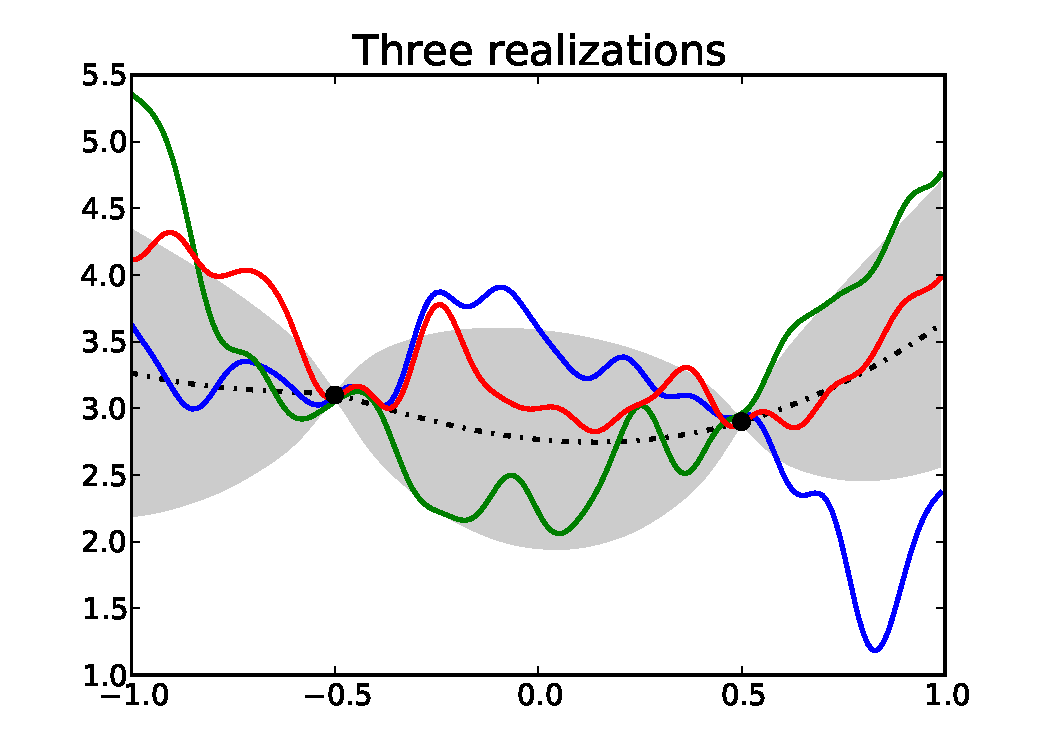
\epsfig{file=figs/basiscov.pdf,width=8cm}
        \caption{Three realizations of an observed Gaussian process whose covariance is an instance of \code{BasisCovariance}. The basis in this case is function \code{fourier_basis} from module \code{cov_funs}. 25 basis functions are used.}
    \label{fig:basiscov}
\end{figure}

It is possible to create random functions from linear combinations of finite sets of basis functions $\{e\}$ with random coefficients $\{c\}$:
\begin{eqnarray*}
    f(x) = M(x) + \sum_{i_0=0}^{n_0-1}\ldots \sum_{i_{N-1}=0}^{n_{N-1}-1} c_{i_1\ldots i_{N-1}} e_{i_1\ldots i_{N-1}}(x), \\
    \{c\}\sim \textup{N}(0,K).
\end{eqnarray*}
It follows that $f$ is a Gaussian process with mean $M$ and covariance defined by
\begin{eqnarray*}
    C(x,y)=\sum_{i_0=0}^{n_0-1}\ldots \sum_{i_{N-1}=0}^{n_{N-1}-1} \sum_{j_0=0}^{n_0-1}\ldots \sum_{j_{N-1}=0}^{n_{N-1}-1} e_{i_0\ldots i_{N-1}}(x) e_{j_0\ldots j_{N-1}}(x) K_{i_0\ldots i_{N-1}, j_0\ldots j_{N-1}},
\end{eqnarray*}
where $K$ is the covariance of the coefficients $c$.

Particularly successful applications of this general idea are:
\begin{description}
    \item[Random Fourier series:] $e_i(x) = \sin(i\pi x/L)$ or $\cos(i\pi x/L)$. See \cite{spanos}.
    \item[Gaussian process convolutions:] $e_i(x) = \exp(-(x-\mu_n)^2)$. See \cite{convolution}.
    \item[B-splines:] $e_i(x) = $ a polynomial times an interval indicator. See \href{http://en.wikipedia.org/wiki/Basis_B-spline}{Wikipedia}'s article.
\end{description}
Such representations can be very efficient when there are many observations in a low-dimensional space, but are relatively inflexible in that they generally produce realizations that are infinitely differentiable. In some applications, this tradeoff makes sense.

This package supports basis representations via the \code{BasisCovariance} class:
\begin{verbatim}
    C = BasisCovariance(basis, cov, **basis_params)
\end{verbatim}
The arguments are:
\begin{description}
    \item[\code{basis}:] Must be an array of functions, of any shape. Each basis function will be evaluated at $x$ with the extra parameters. The basis functions should obey the same calling conventions as mean functions: return values should have shape \code{x.shape[:-1]} unless $x$ is one-dimensional, in which case return values should be of the same shape as \code{x}. Note that each function should take the entire input array as an argument.
    \item[\code{cov}:] An array whose shape is either:
        \begin{itemize}
            \item Of the same shape as \code{basis}. In this case the coefficients are assumed independent, and \code{cov[i[0],...,i[N-1]]} (an $N$-dimensional index) simply gives the prior variance of the corresponding coefficient.
            \item Of shape \code{basis.shape * 2}, using \proglang{Python}'s convention for tuple multiplication. In this case \code{cov[i[0],...,i[N-1], j[0],...,j[N-1]]} (a $2N$-dimensional index) gives the covariance of $c_{i_0\ldots i_{N-1}}$ and $c_{j_1\ldots j_{N-1}}$.
        \end{itemize}
        Internally, the basis array is ravelled and this covariance tensor is reshaped into a matrix. This input convention makes it easier to keep track of which covariance value corresponds to which coefficients. The covariance tensor must be symmetric (\code{cov[i[0],...,i[N-1], j[0],...,j[N-1]]} $=$ \code{cov[j[0],...,j[N-1], i[0],...,i[N-1]]}), and positive semidefinite when reshaped to a matrix.
    \item[\code{basis_params}:] Any extra parameters required by the basis functions.
\end{description}

\section{Separable bases}

Many bases, such as Fourier series, can be decomposed into products of functions as follows:
\begin{eqnarray*}
    e_{i_0\ldots i_{N-1}}(x) = \prod_{j=0}^{N-1}e_{i_j}^j(x)
\end{eqnarray*}
Basis covariances constructed using such bases can be represented more efficiently using \code{SeparableBasisCovariance} objects. These objects are constructed just like \code{BasisCovariance} objects, but instead of an $n_0\times \ldots \times n_{N-1}$ array of basis functions they take a nested lists of functions as follows:
\begin{verbatim}
    basis = [ [e[0][0], ... ,e[0][n[0]-1]]
                       ...
              [e[N-1][0], ... ,e[N-1][n[N-1]-1]] ].
\end{verbatim}
For an $N$-dimensional Fourier basis, each of the \code{e}'s would be a sine or cosine; frequency would increase with the second index. As with \code{BasisCovariance}, each basis needs to take the entire input array \code{x} and \code{basis_params} as arguments. See \code{fourier_basis} in \code{examples/gp/basiscov.py} for an example.

\subsection{Example}

Once created, a \code{BasisCovariance} or \code{SeparableBasisCovariance} object behaves just like a \code{Covariance} object, but it and any \code{Mean} and \code{Realization} objects associated with it will take advantage of the efficient basis representation in their internal computations. An example of \code{SeparableBasisCovariance} usage is given in \code{pymc/examples/gp/basis_cov.py}. Compare its output in figure \ref{fig:basiscov} to that of \code{pymc/examples/gp/observation.py}.
 

\chapter{Incorporating Gaussian processes in larger probability models with PyMC}\label{cha:PyMC}
This chapter will show you how to build and fit statistical models that go beyond simple nonparametric regression.

\section{Gaussian process submodels}

\subsection{The \texttt{GaussianProcess} class} 

\section{Step methods}
Some general ideas
\subsection{The \texttt{GPEvaluationGibbs} class} 
\subsection{Step methods that handle parents of Gaussian processes}
\subsubsection{Choosing a mesh}  



\section{Example: A simple extension of nonparametric regression}\label{sub:BasicMCMC}
The files \file{examples/gp/PyMCModel.py} and \file{examples/gp/MCMC.py} show Gaussian process submodels and the step methods listed above in action. The probability model created by \file{PyMCModel.py} is illustrated as a directed acyclic graph in figure \ref{fig:unobservedModel}. If you comment the last line, $f_eval$ will be handled by a default \class{GPParentAdaptiveMetropolis} instance. If you leave it uncommented, $f$ will be handled by a \class{GPEvaluationGibbs} instance.

The main script \file{examples/gp/MCMC.py} is mostly devoted to plotting, and its output is shown in figure \ref{fig:MCMCOutput} for both the \class{GPEvaluationMetropolis} and \class{GPParentAdaptiveMetropolis} step methods.

\begin{figure}
    \centering
        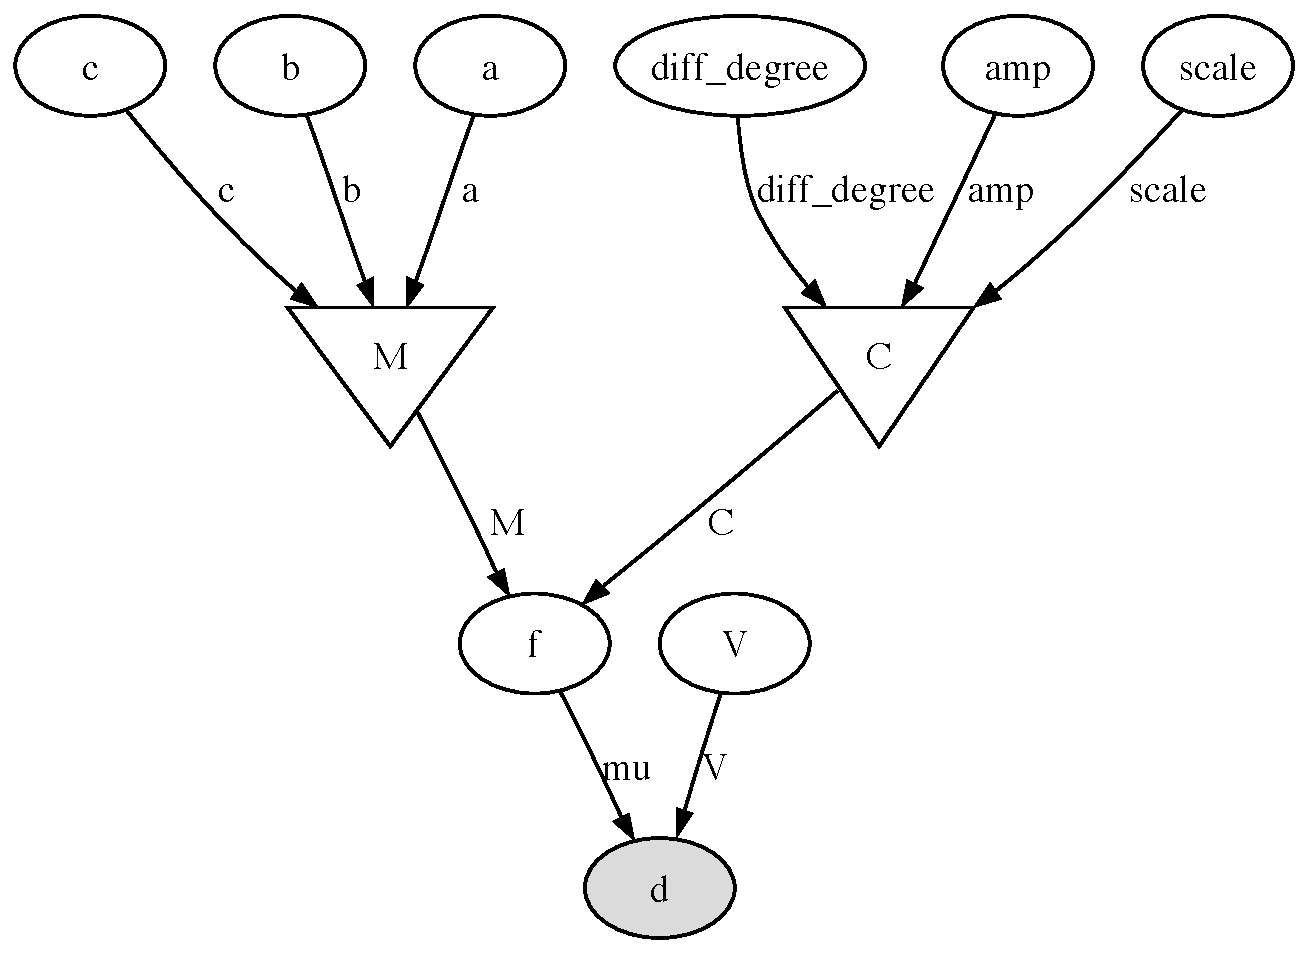
\epsfig{file=figs/unobservedModel.pdf, width=10cm}
    \caption{The PyMC-generated directed acyclic graph representation of the extended nonparametric regression model created by \textsf{`examples/gp/PyMCModel.py'} . Ellipses represent \class{Stochastic} objects (variables whose values are unknown even if their parents' values are known), triangles represent \class{Deterministic} objects (variables whose values can be determined if their parents' values are known), and rectangles represent \class{Stochastic} objects with the \member{isdata} flag set to \member{True} (data). Arrows point from parent to child, and arrow labels show the name assigned to the parent by the child. For instance, \class{C} considers \class{C_amp} to be its `\class{amp}' parameter.}
    \label{fig:unobservedModel}
\end{figure}

\begin{figure}
    \centering
        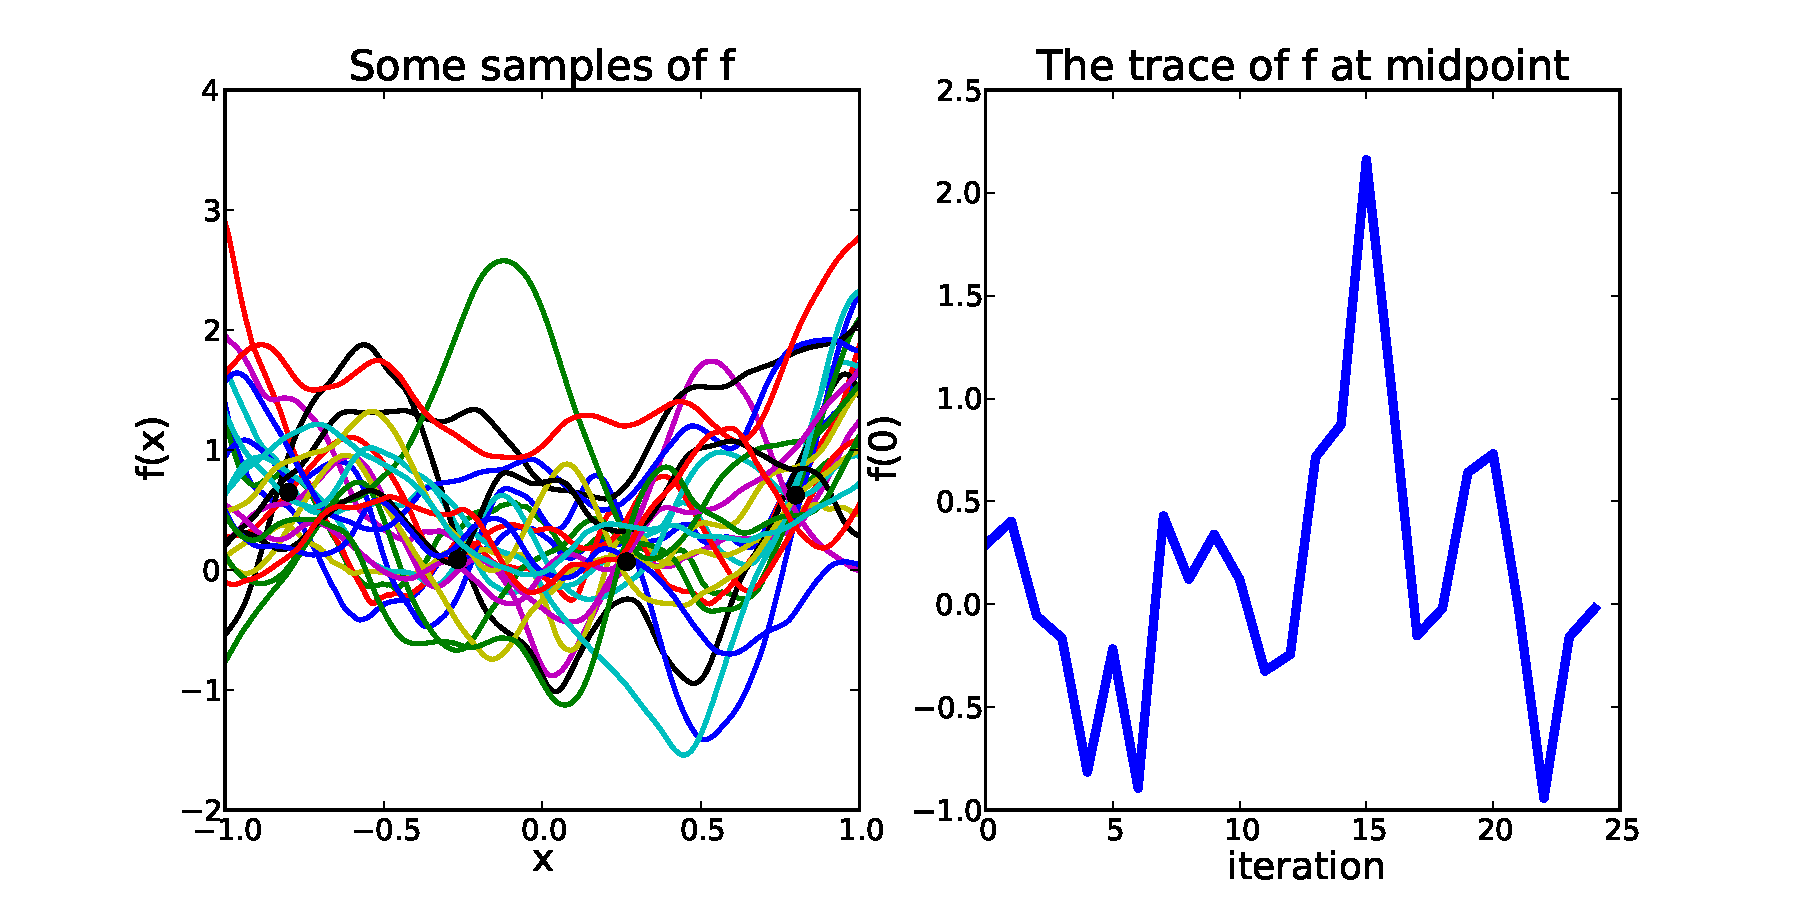
\epsfig{file=figs/gibbsSamples.pdf,width=10cm}
        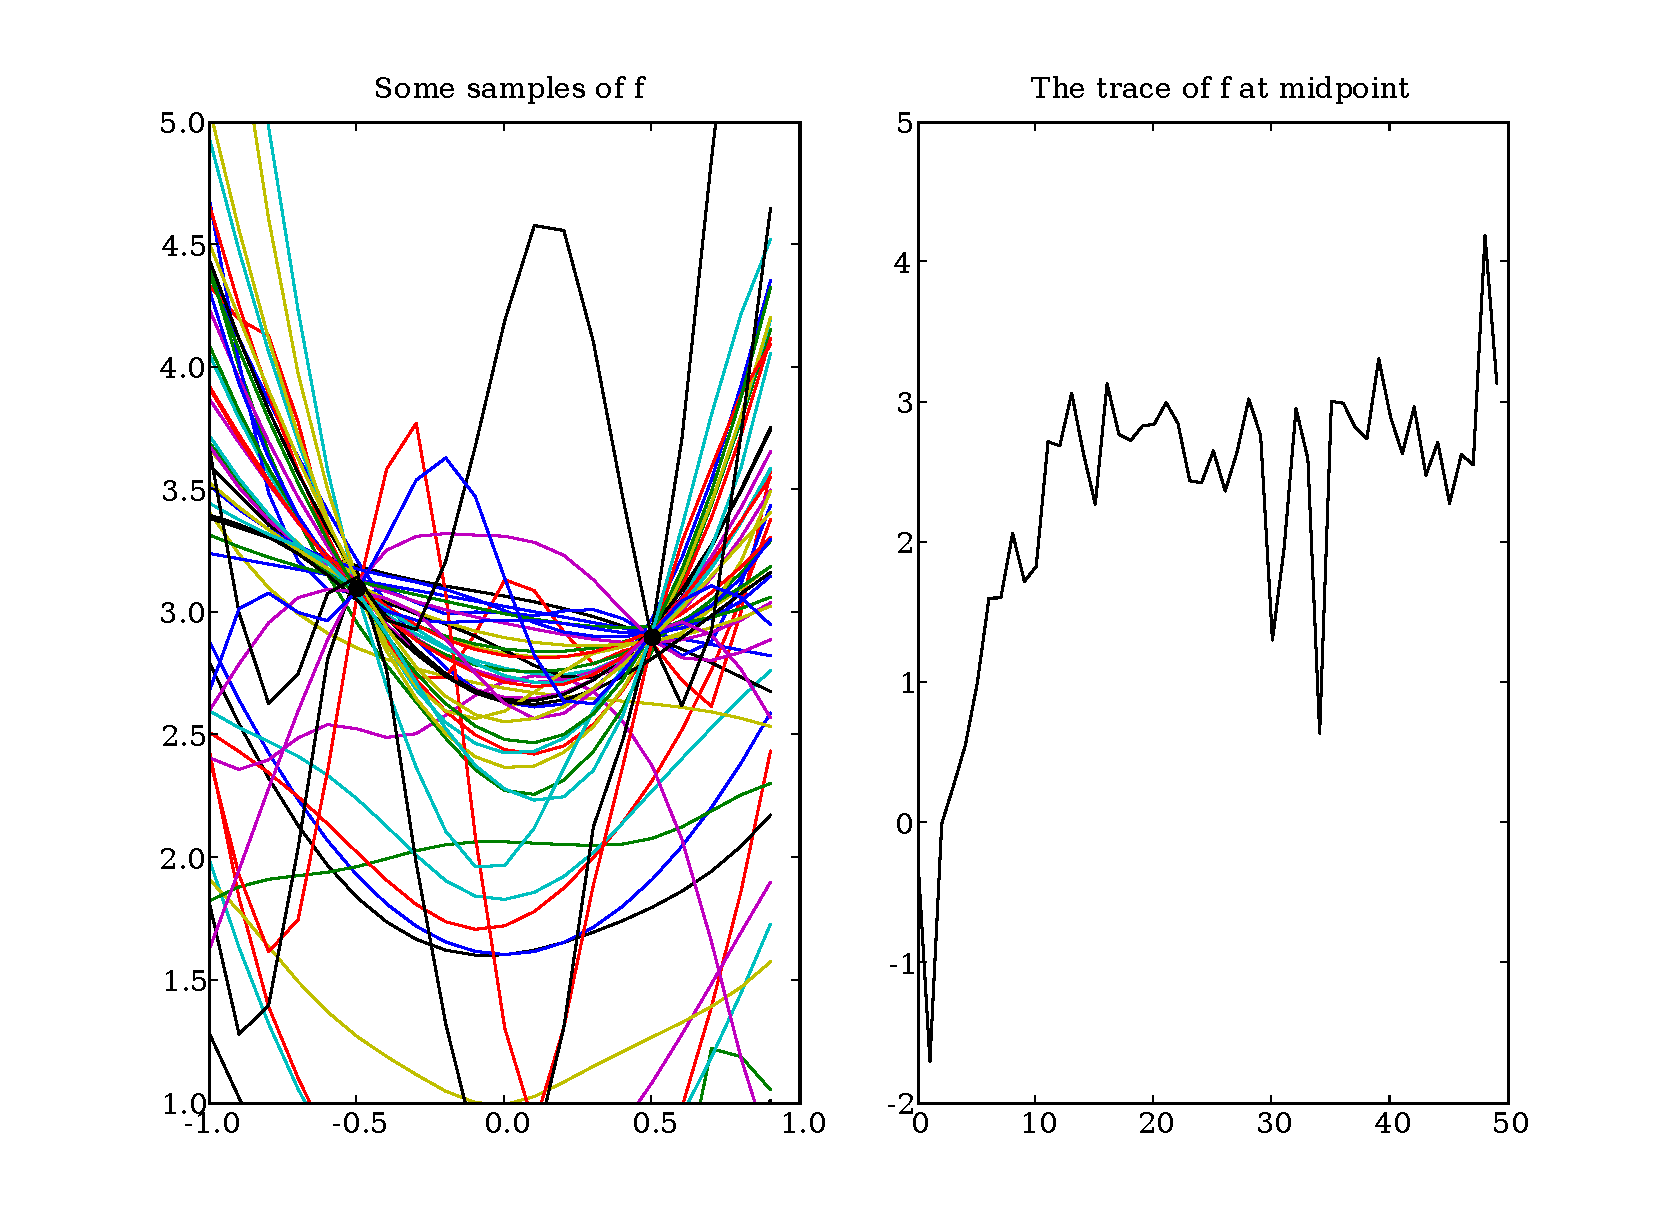
\epsfig{file=figs/metroSamples.pdf,width=10cm}
    \caption{The output of {\sffamily `examples/gp/MCMC.py'} using the \class{GPEvaluationGibbs} (top) and \class{GPParentAdaptiveMetropolis} (bottom) step methods. Note that the Metropolis samples take several iterations to `burn in' to their dense support, whereas the Gibbs samples jump there more or less immediately.
    \label{fig:MCMCOutput}
\end{figure}

\section{Example: Munch, Kottas and Mangel's stock-recruitment study}\label{sub:MMKMCMC}

\begin{figure}
    \centering
        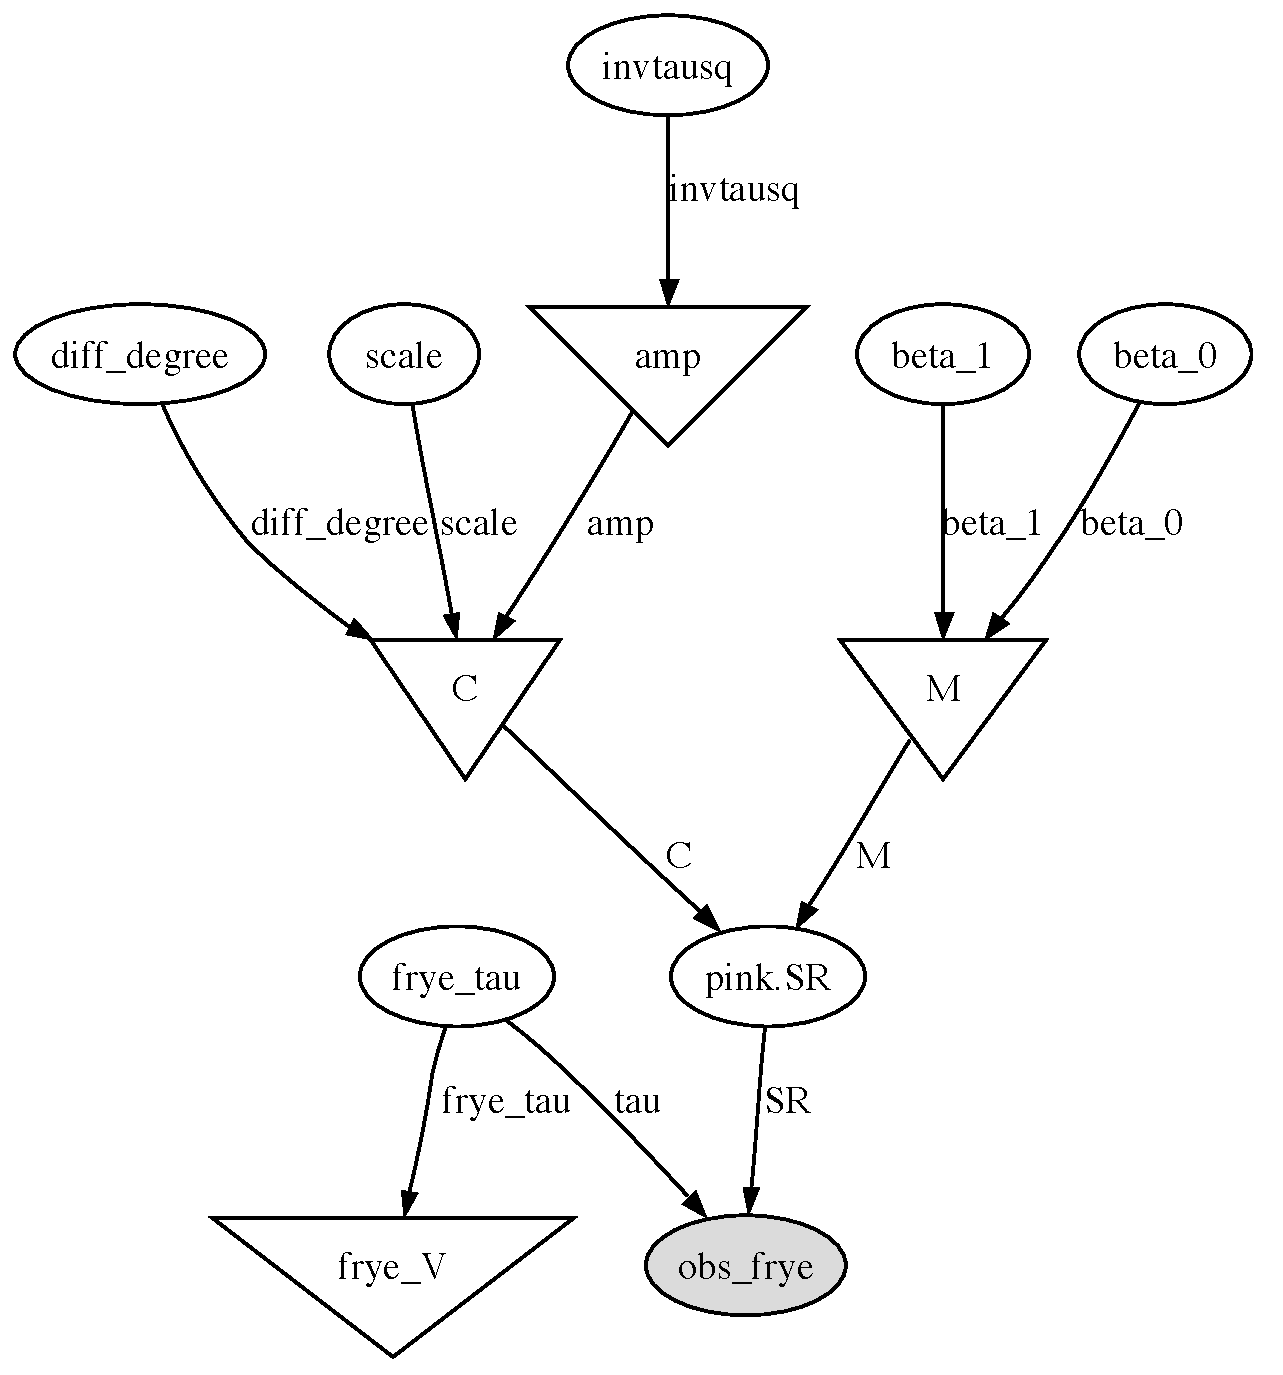
\epsfig{file=figs/MKMsalmon.pdf, width=10cm}
    \caption{A PyMC-generated directed acyclic graph representation of the probability model in (\ref{eqn:MMKModel}), which is implemented in file \textsf{`examples/gp/more_examples/MKMSalmon/salmon_sampler.py'}. A very similar probability model was used by Munch, Kottas and Mangel to infer stock-recruitment functions for three salmonid species. The label `\texttt{pink.SR}' indicates that this particular model corresponds to the pink salmon (\emph{Onchorhynchus gorbuscha}) data. Note that two coordinate transformations are implemented using PyMC deterministic variables. This technique can help lazy programmers avoid transforming priors by hand, and in less trivial cases it can save computation by caching the transformed parameters.}
    \label{fig:MMKsalmonmodel}
\end{figure}

\begin{figure}
    \centering
        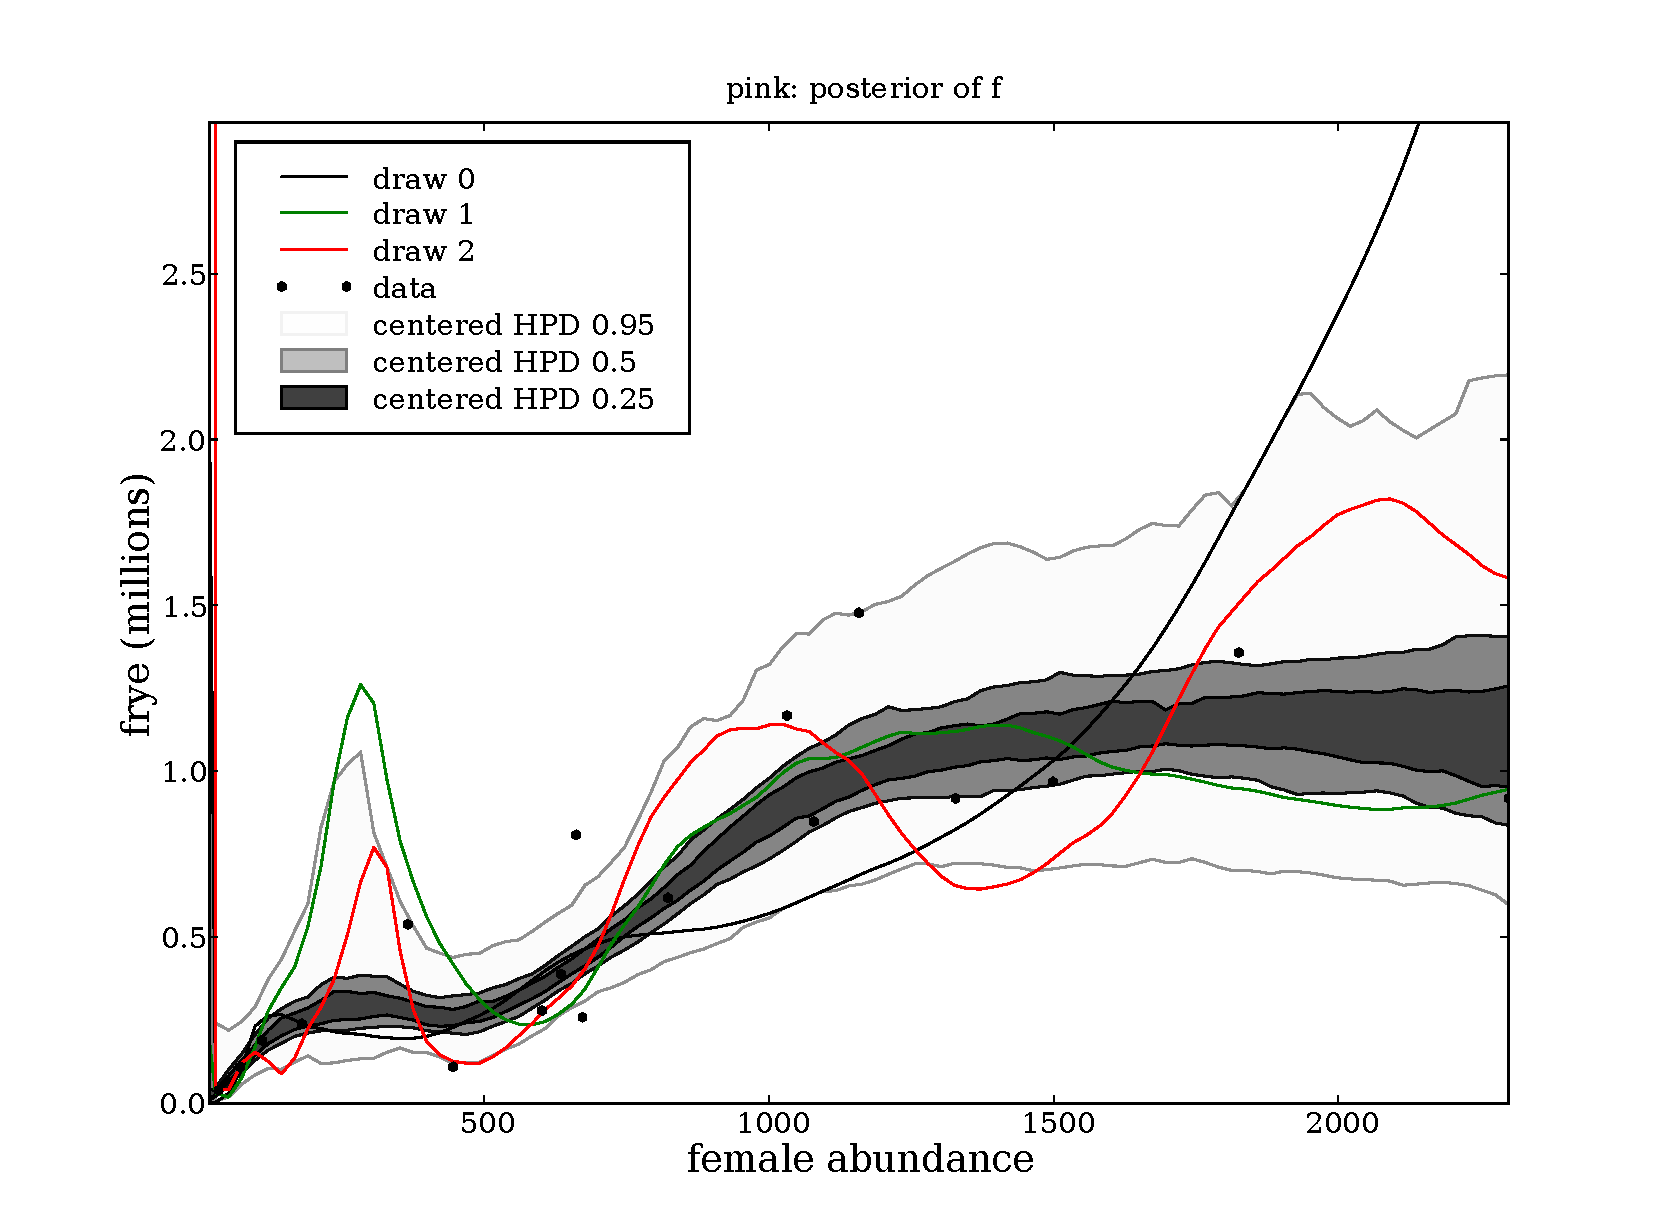
\epsfig{file=figs/pinkfpost.pdf, width=10cm}
    \caption{The posterior of the stock-recruitment function for pink salmon (\emph{Onchorhynchus gorbuscha}). The data are shown as heavy black dots. The centered 95\%, 50\% and 25\% posterior probability intervals are shown as shaded regions. Three draws from the posterior are plotted.}
    \label{fig:pinkfpost}
\end{figure}

\begin{figure}
    \centering
        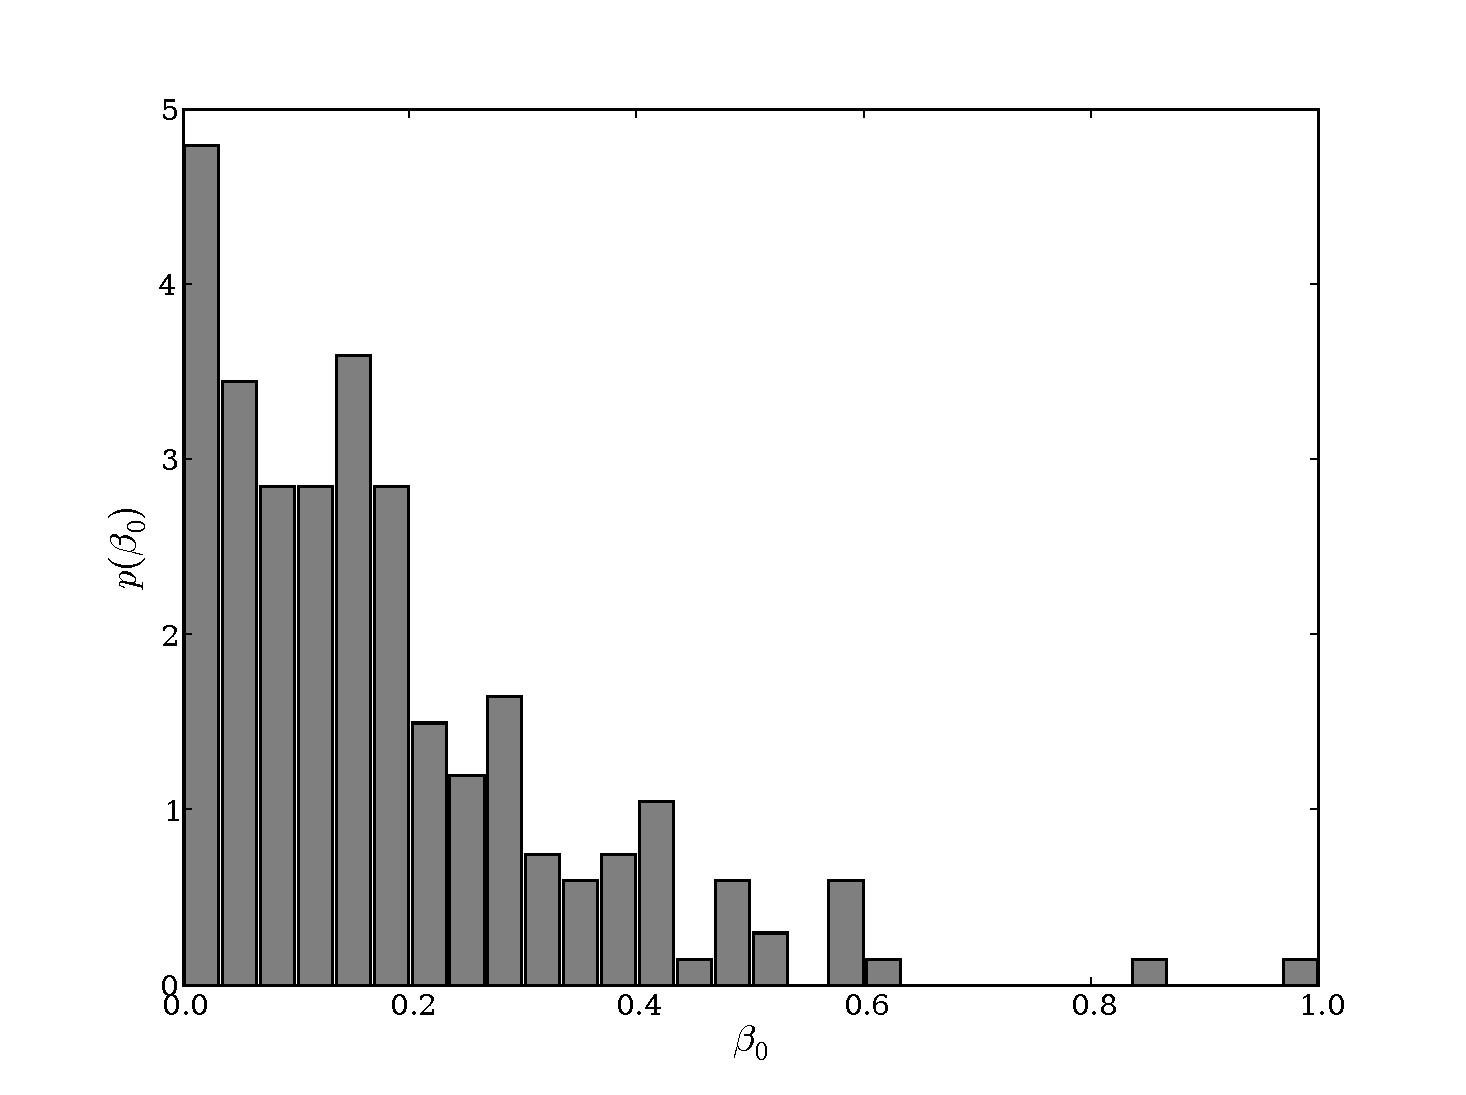
\epsfig{file=figs/pinkbeta0post.pdf, width=5cm}
        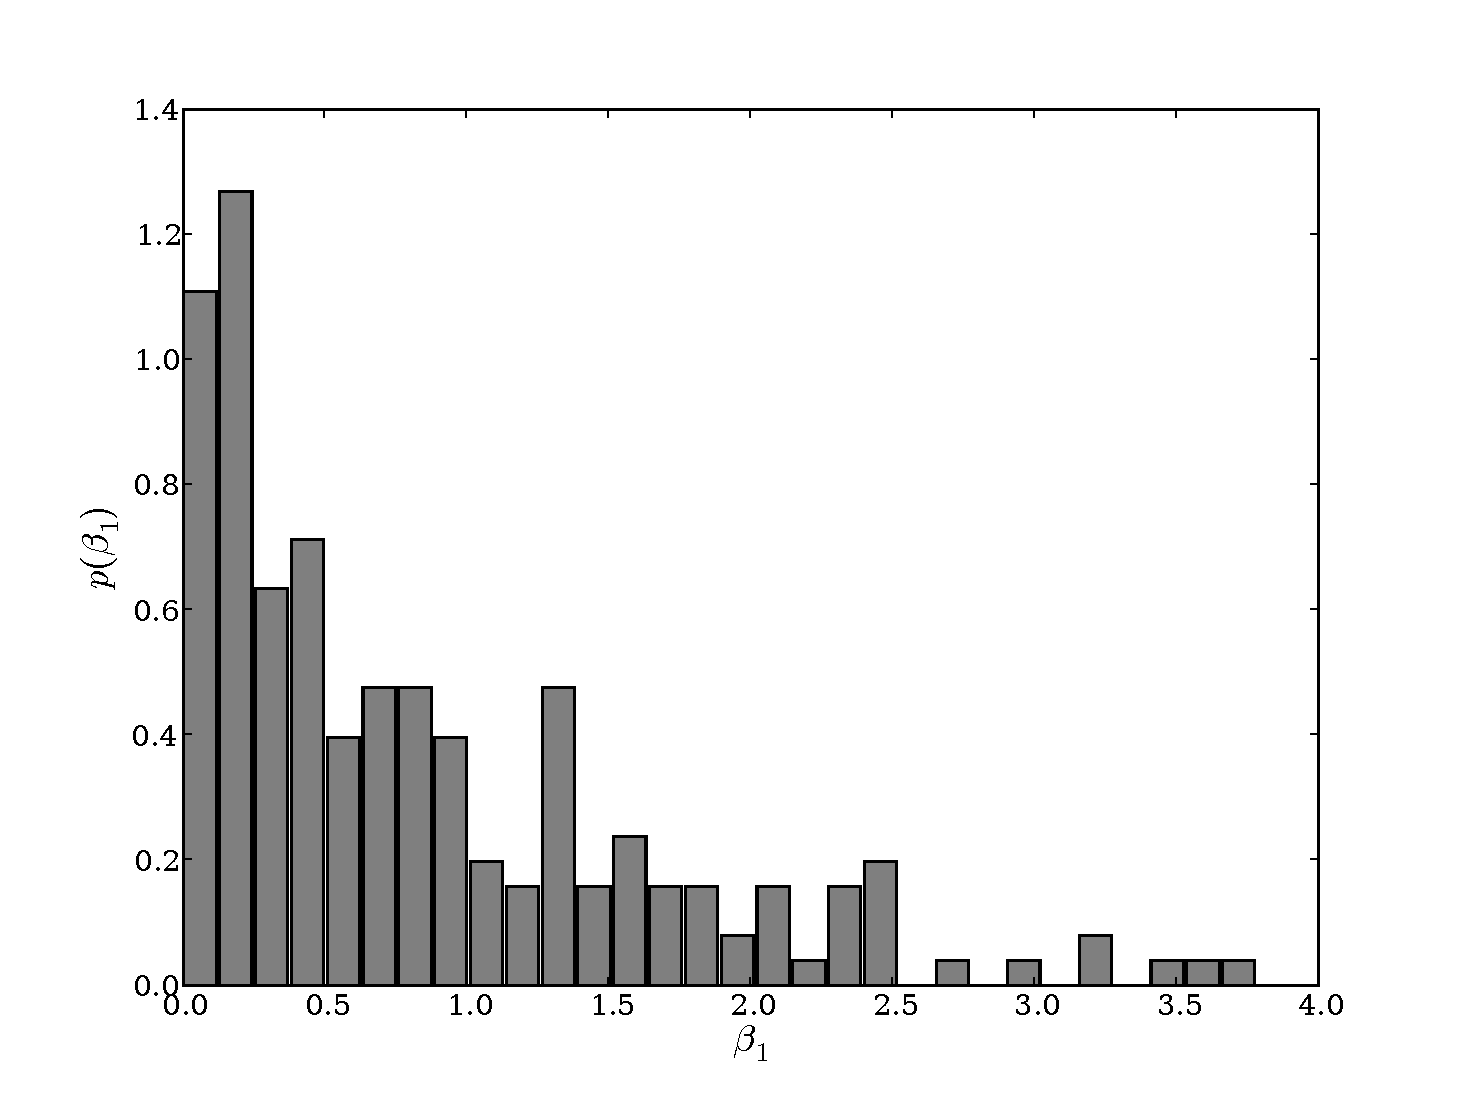
\epsfig{file=figs/pinkbeta1post.pdf, width=5cm}
        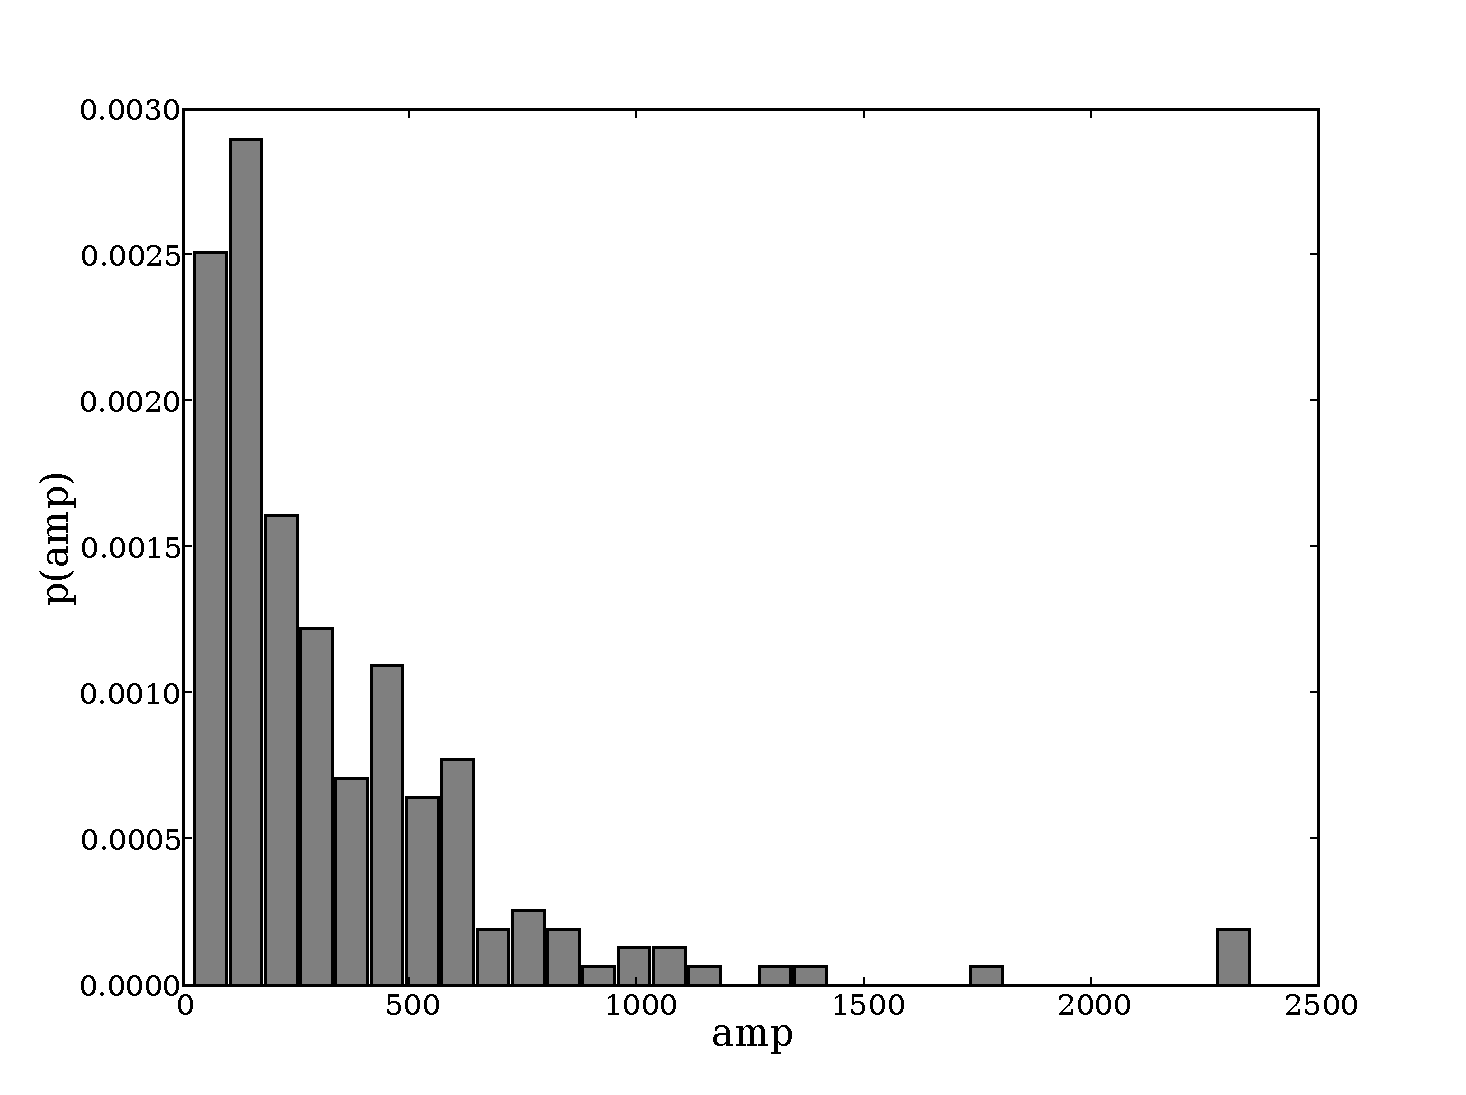
\epsfig{file=figs/pinkamppost.pdf, width=5cm}
        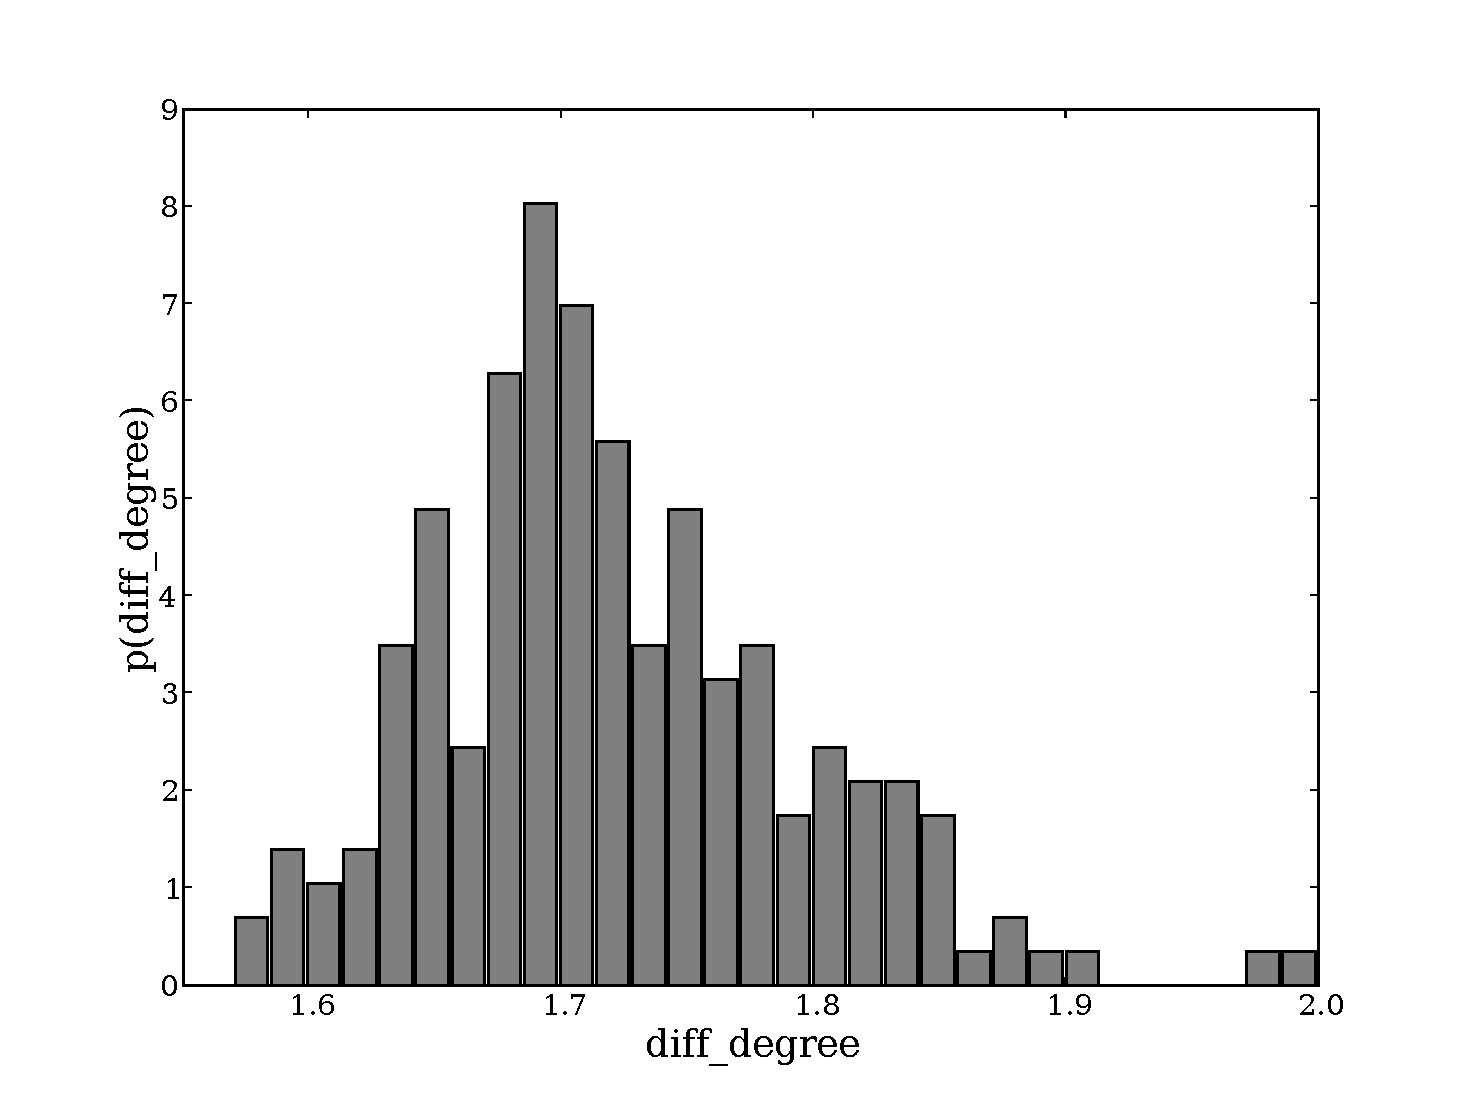
\epsfig{file=figs/pinkdiffdegreepost.pdf, width=5cm}
        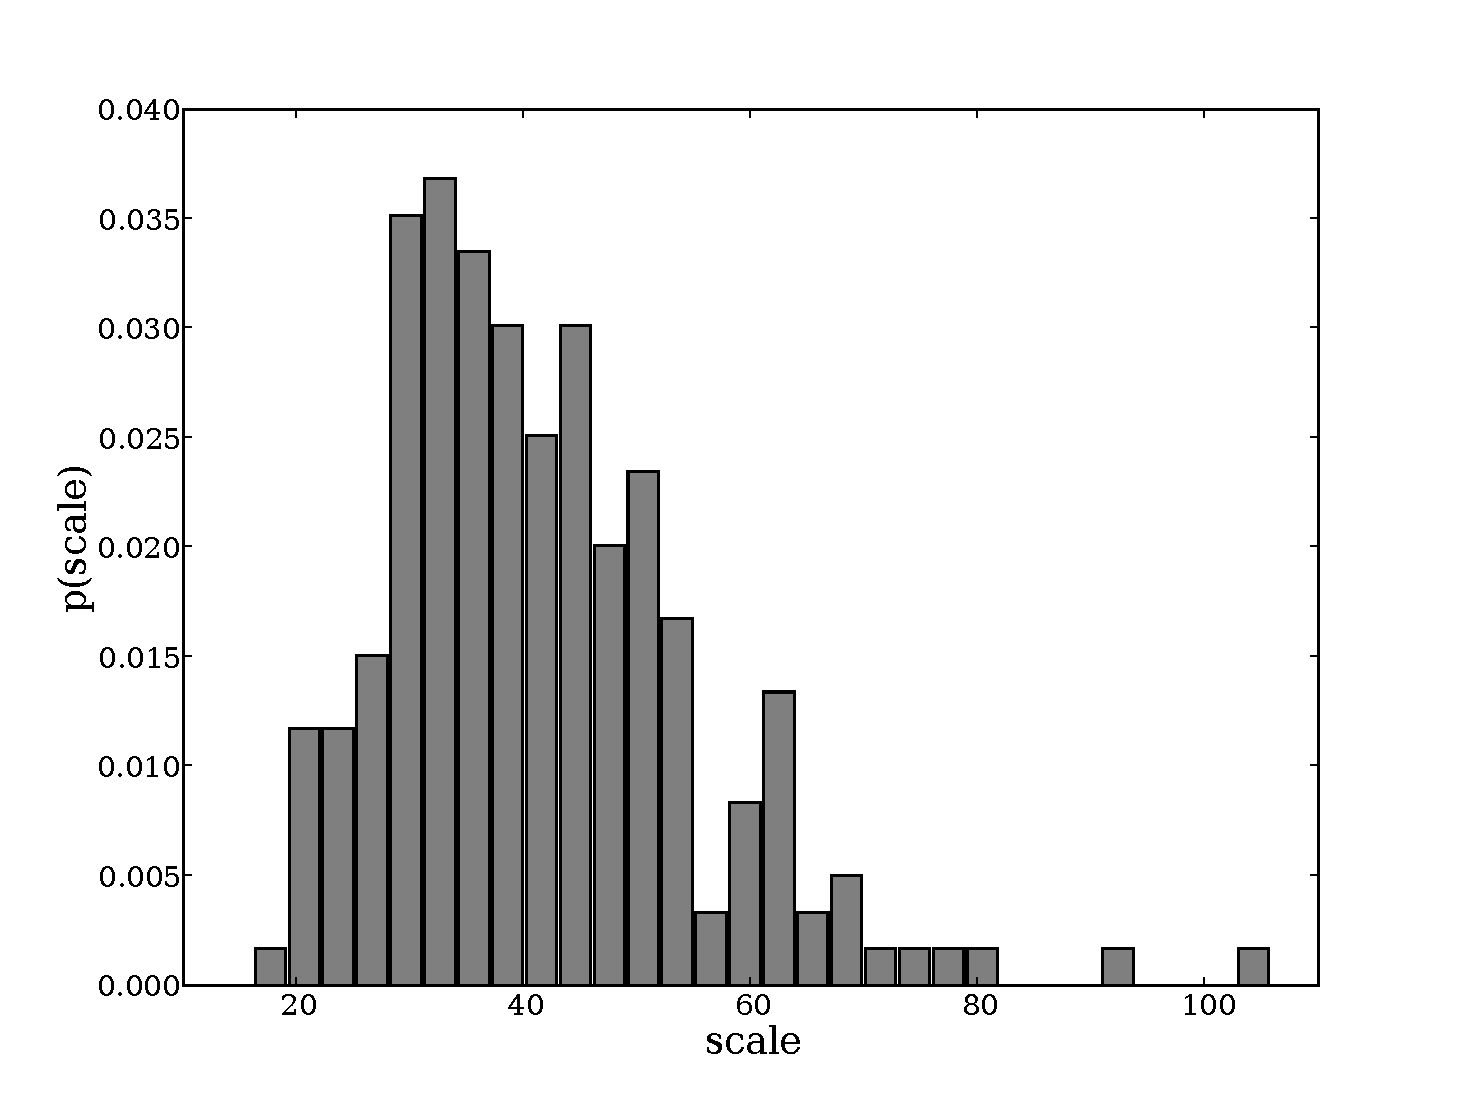
\epsfig{file=figs/pinkscalepost.pdf, width=5cm}
        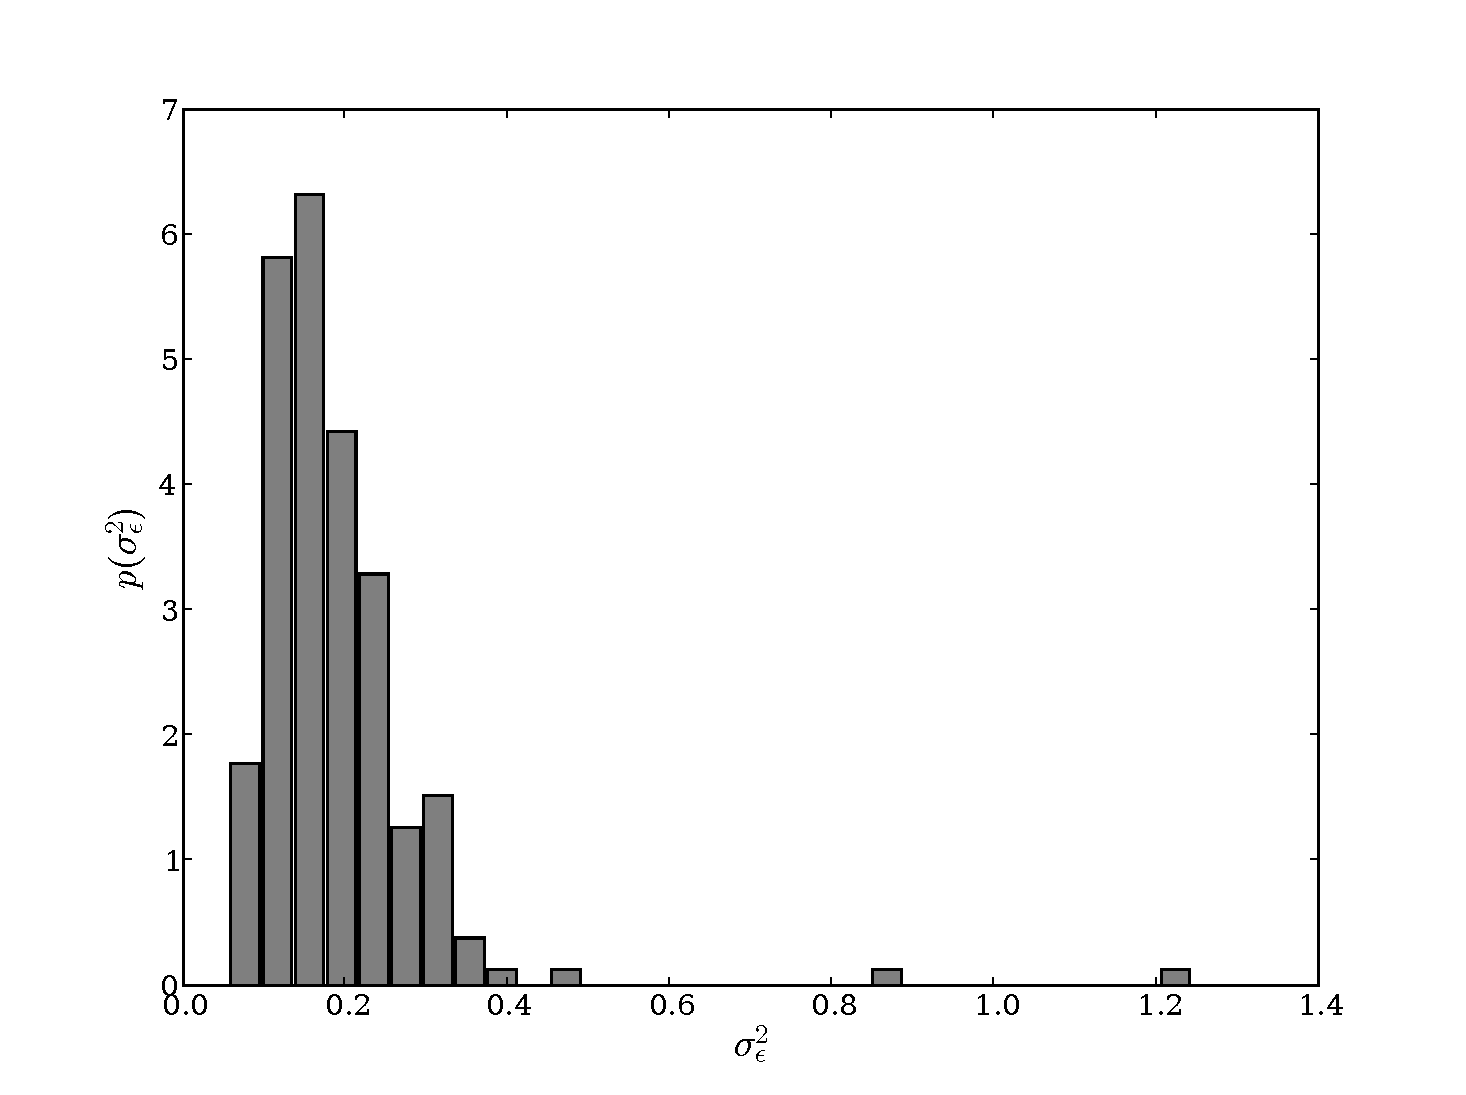
\epsfig{file=figs/pinkVpost.pdf, width=5cm}
    \caption{The marginal posterior distributions of the mean and covariance parameters of the stock-recruitment function for pink salmon (\emph{Onchorhynchus gorbuscha}).}
    \label{fig:pinkparams}
\end{figure}

We now have the tools to duplicate Munch, Kottas and Mangel's \cite{mmk} stock-recruitment results. The full probability we'll use follows. It is like Munch, Kottas and Mangel's probability model, but we will use a Mat\`ern covariance function. Here \texttt{SR} is the stock-recruitment function, C is its covariance and M is its mean.
\begin{equation}
    \label{eqn:MMKModel}
    \begin{array}{ll}
        \texttt{frye}[i] \stackrel{\tiny{\textup{ind}}}{\sim} \textup{N}(exp(\mathtt{SR}(\log(\mathtt{abundance}[i]))), V),& i=1\ldots n\\
        \texttt{SR}\sim \textup{GP}(M,C)& \\
        M:x\rightarrow \beta_0+\beta_1 \log(x)&\\
        C:x,y\rightarrow \texttt{matern.euclidean}(x,y;\ \texttt{diff_degree},\texttt{amp},\texttt{scale})&\\
        V,\ \beta_0,\ \beta_1,\ \texttt{diff_degree},\ \texttt{amp},\ \texttt{scale} \sim \texttt{priors}.&
    \end{array}
\end{equation}
The `priors' can be found by reading their paper (except the prior on \texttt{diff_degree}, which I chose based on what seems reasonable to me) or by reading the file \file{examples/more_examples/MMKSalmon/salmon_sampler.py}. This file contains a PyMC \class{MCMC} subclass called \class{SalmonSampler}, which reads in the data, creates a probability model incorporating the data, and provides some plotting methods.

Note that this model differs from the model in section \ref{sub:MMKregression} in that we're putting a Gaussian process prior on the stock-recruitment function in log-log space, so conditioning its value at zero isn't an option.

The probability model \class{SalmonSampler} creates is visualized as a directed acyclic graph in figure \ref{fig:MMKsalmonmodel}. Munch, Kottas and Mangel specify priors for $\texttt{amp}^{-2}$ and $V^{-1}$, and I've used PyMC deterministic variables to conveniently implement the transformations rather than changing variables manually. The posterior distribution of \texttt{SR} for the pink salmon (\emph{Onchorhynchus gorbuscha}) is shown in figure \ref{fig:pinkfpost}, and the posterior of the mean and covariance parameters for the same species are shown in figure \ref{fig:pinkparams}.


\chapter{Old stuff} 

\section{The \class{GP} class}
\class{GP} is a subclass of the PyMC \class{Stochastic} class whose value attribute is a \class{Realization} instance. Its init method takes the following arguments:
\begin{description}
    \item[$M$:] A mean object or mean-valued deterministic variable.
    \item[$C$:] A covariance object or covariance-valued deterministic variable.
    \item[\texttt{mesh=None}:] An array or an array-valued variable.
    \item[\texttt{init_mesh_vals=None}:] An optional vector of initial values for the value attribute's evaluation on \texttt{mesh}.
    \item[\texttt{mesh_eval_isdata=False}:] If \texttt{True}, the value attribute's evaluation on \texttt{mesh} is fixed at \texttt{init_mesh_vals}.
    \item[\texttt{doc, name, trace, cache_depth, verbose}:] Optional arguments that are passed directly to \code{Stochastic.\_\_init\_\_}. See PyMC's documentation.
\end{description}

\texttt{GP} instances have a log-probability attribute like any PyMC stochastic variable, but there is an important difference: If the value attribute is a realization called $f$, the log-probability attribute gives $p(f\texttt{(mesh))}|M,C)$. In other words, the log-probability attribute only cares about $f$'s evaluation on \texttt{mesh}. The reason is simple: it would be expensive and difficult to assign something like a log-density to entire realizations in most cases.

\section{The \class{GPMetropolis} and \class{GPParentMetropolis} step methods}

The a price of the `cop-out' of computing \texttt{GP}s' log-probabilities based only on their evaluation on a mesh is that the Metropolis-Hastings algorithm doesn't apply. \texttt{GPMetropolis} and \texttt{GPParentMetropolis} employ a strategy that will be described informally here.

Although they're contained in the same object, think about splitting the value $f$ of a \texttt{GP} into two pieces: an array $f$\texttt{(mesh)}, and a function $\tilde f$ defined on all values not in \texttt{mesh}. Denote the parents of the \class{GP} by $P$ and the children by $K$.

\section{GPMetropolis}
The Metropolis-Hastings acceptance ratio for a proposed value $f_p$ can be written as follows:
\begin{eqnarray*}
    \frac{p(K|\tilde f_p, f_p(\mathtt{mesh}))\ p(\tilde f_p|f_p(\mathtt{mesh}), P)\ p(f_p(\mathtt{mesh}) | P)\ q(\tilde f|f(\mathtt{mesh}))\ q(f(\mathtt{mesh}))}{p(\mathtt{K}|\tilde f, f(\mathtt{mesh}))\ p(\tilde f|f(\mathtt{mesh}), P)\ p(f(\mathtt{mesh}) | P)\ q(\tilde f_p|f(\mathtt{mesh}))\ q(f_p(\mathtt{mesh}))},
\end{eqnarray*}
where $q$ denotes proposal densities. We want to avoid computing all terms with $\tilde f$ or $\tilde f_p$ in the consequent position:
\begin{eqnarray*}
    p(\tilde f_p|f_p(\texttt{mesh}), P),\\ q(\tilde f|f(\texttt{mesh})),\\ p(\tilde f|f(\texttt{mesh}), P),\\ q(\tilde f_p|f(\texttt{mesh})),
\end{eqnarray*}
but all other terms are fine. We can make these terms cancel by choosing our proposal distribution as follows:
\begin{eqnarray*}
    q(\tilde f_p|f(\texttt{mesh})) = p(\tilde f_p|f_p(\texttt{mesh}), P).
\end{eqnarray*}
In other words, if we propose $\tilde f$ from its prior distribution conditional on $f(\texttt{mesh})$ and its parents whenever we propose $f(\texttt{mesh})$, we don't have to worry about computing the intractable terms. This is what \class{GPMetropolis} does.

\class{GPMetropolis} reports its competence to handle \texttt{GP} instances as \texttt{3}, so it will be chosen as the default handler. Its init method takes the following arguments:
\begin{description}
    \item[\texttt{stoch}:] The \class{GPMetropolis} instance to be handled.
    \item[\texttt{scale=.1}:] $f(\texttt{mesh})$ will be proposed from a random-walk multivariate normal distribution with covariance equal to \texttt{C(mesh, mesh * scale * adaptive_scale_factor)}, where C is the covariance-valued parent and \texttt{adaptive_scale_factor} is the adaptive scaling factor, which is updated when \texttt{self.tune()} is called.
    \item[\texttt{verbose = 0}:] An integer from 0 to 3 indicating the preferred verbosity level.
\end{description}

\section{GPParentMetropolis}
Similarly, the Metropolis-Hastings acceptance ratio for a proposed value $P_p$ of the parents \emph{and} a proposed value $\tilde f_p$ for the function off the mesh is as follows:
\begin{eqnarray*}
    \frac{p(K|\tilde f_p)\ p(\tilde f_p|f(\texttt{mesh}), P_p)\ p(f(\texttt{mesh}) | P_p)\ q(\tilde f_p|f(\texttt{mesh}),f_p, P_p)\ q(P)}{p(K|\tilde f)\ p(\tilde f|f(\texttt{mesh}), P)\ p(f(\texttt{mesh}) | P)\ q(\tilde f_p|f(\texttt{mesh}),f)\ q(P_p)}
\end{eqnarray*}
By choosing the same proposal distribution for $\tilde f$ as above, we again avoid having to compute the intractable terms. In other words, every time a value is proposed for a \class{GP}'s parent, a value must be proposed for the \class{GP}  conditional on its value's evaluation on its mesh, and the prior probability of the \class{GP}'s children must be included in the acceptance ratio.

To implement this strategy, \class{GPParentMetropolis} wraps an instance of a \class{Metropolis} subclass. It replaces its host class's \texttt{propose} and \texttt{reject} methods with special methods that call the host's native methods, and then propose and reject values for $\tilde f$ conditional on \texttt{f(mesh)}. \class{GPParentMetropolis} also adds the \texttt{GP}'s children to its host method's children, so that the likelihood term $p(K|\tilde f)$ is included in the acceptance ratio.

\class{GPParentMetropolis} reports its competence to handle parents of \class{GP} instances as \texttt{3}, so it will be chosen as the default handler. However, its init method will choose the host method by checking the step method registry for a method that would be competent to handle the parent if it had ordinary children. Its init method takes the following arguments:
\begin{description}
    \item[\texttt{stochastic}:] The stochastic variable to handle. Must be a parent of a \class{GP} instance.
    \item[\texttt{scale = 1.}:] This parameter will be passed to the host method's init method.
    \item[\texttt{verbose = 0}:] An integer from 0 to 3 indicating the preferred verbosity level.
\end{description}

This scheme works if $K$ depends on $P$ and if $P$ has children other than the \class{GP}, though these possibilites aren't included in the rejection ratio above.

\section{Choosing a mesh} A useful mental model for these step methods is as follows: The mesh points of a \class{GP} instance are the points where you `grab' its value to propose it. If the variable's mesh is \texttt{None}, its value will be proposed from its prior, and rejection rates are likely to be quite large. If the mesh is too dense, on the other hand, computation of the log-probability will be expensive (it scales as the cube of the number of points in the mesh). If the mesh is so dense that \texttt{C(mesh, mesh)} is numerically singular, an error will be raised in the init method. This continuum is illustrated in figure \ref{fig:meshpropose}. Finding the happy medium will require some experimentation.

Another important point to bear in mind is that if the \texttt{GP}'s children depend on its value only via its evaluation on the mesh, the likelihood terms $p(K|\tilde f_p)$ and $p(K|\tilde f)$ will cancel. In other words, if the mesh is chosen so that $p(K|f)=p(K|f(\texttt{mesh}))$ then the proposed value of $\tilde f$ will have no bearing on the acceptance probability of the proposed value of \texttt{f(mesh)} or of the parents P. Such a mesh choice will generally improve the acceptance rate.

\begin{figure}
    \centering
        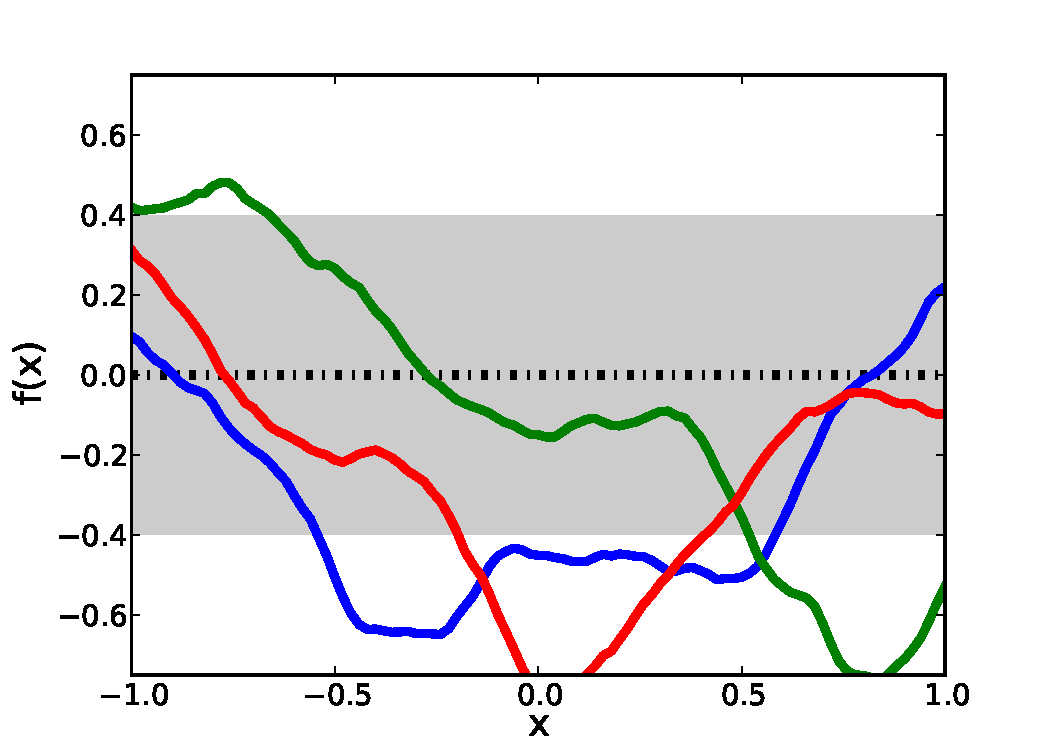
\epsfig{file=figs/nomeshpropose.pdf,width=9cm}
        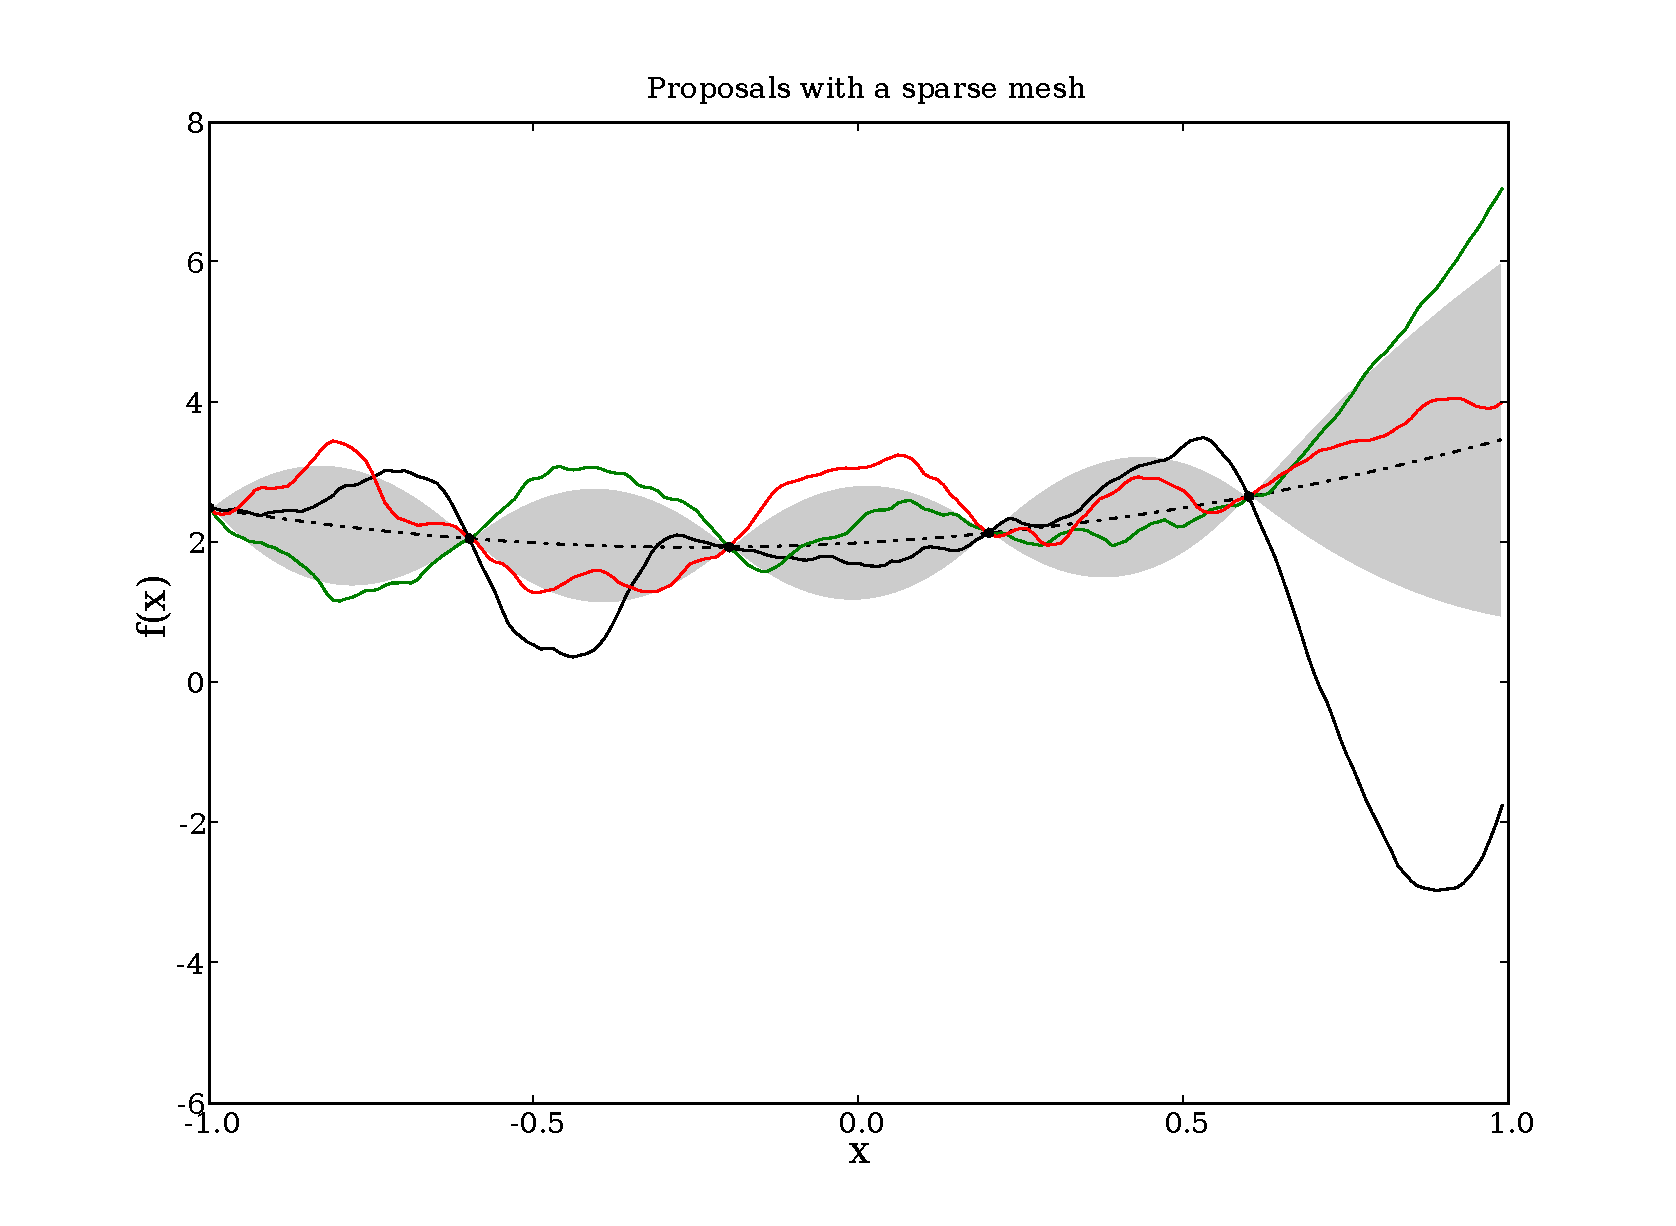
\epsfig{file=figs/lightmeshpropose.pdf,width=9cm}
        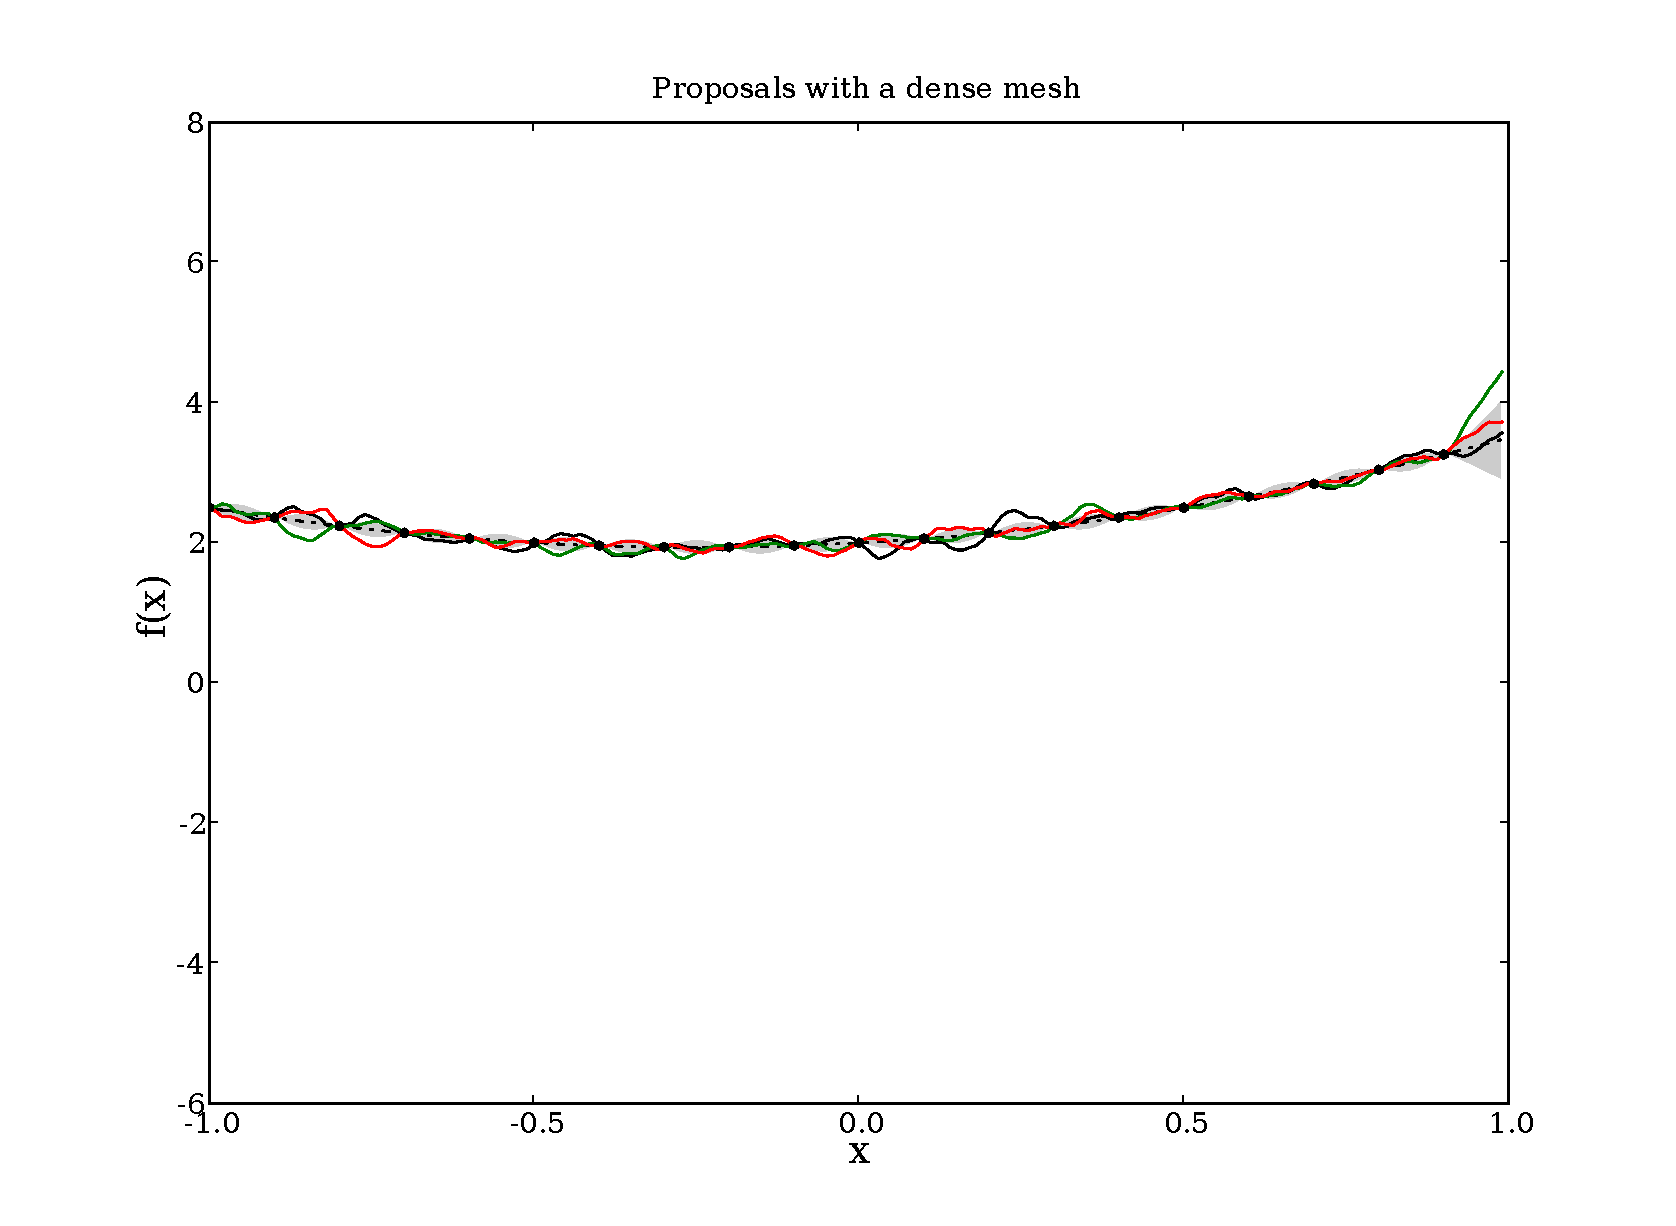
\epsfig{file=figs/densemeshpropose.pdf,width=9cm}
    \caption{Several possible proposals of $\tilde f$ (curves) given proposed values for $f(\texttt{mesh})$ (heavy dots) with no mesh (top), a sparse mesh (middle), and a dense mesh (bottom). Proposal distributions' envelopes are shown as shaded regions, with means shown as broken lines. With no mesh, $\tilde f$ is being proposed from its prior and the acceptance rate will be very low. A denser mesh permits a high degree of control over $\tilde f$, but computing the log-probability will be more expensive.}
    \label{fig:meshpropose}
\end{figure}


\section{The \class{GPNormal} step method}
As we've already seen in other contexts, a \class{GP}'s full conditional distribution is a Gaussian process if its Markov blanket is described by the following probability model:
\begin{eqnarray*}
    K_i |f \sim \textup{N}(f(o_i), V_i) & i=0\ldots n-1\\
    f|M,C\sim\textup{GP}(M,C)
\end{eqnarray*}
In other words, each of its children $K_i$ is normally distributed with variance $V_i$ and mean equal to $f(o_i)$, where $o_i$ is an arbitrary mesh.

In this case, a \texttt{GP} instance $f$ can be handled by the Gibbs step method \class{GPNormal}, which will have much better mixing properties that \class{GPMetropolis}. Its init method takes the following parameters:
\begin{description}
    \item[$f$:] The \texttt{GP} instance to be handled.
    \item[\texttt{obs_mesh:}] An array or array-valued variable giving the observation mesh $o$.
    \item[\texttt{obs_V}:] An array or array-valued variable giving the observation variance $V$.
    \item[\texttt{obs_vals}:] An array or array-valued variable giving the concatenation of the values of the children $K_i$.
\end{description}

\class{GPNormal} doesn't register itself, so it will never be assigned as a default handler. This may change eventually.

\class{GPNormal} doesn't care about $f$'s mesh, because it never has to evaluate $f$'s log-probability. However, a good choice of mesh is important because it will used by the \class{GPParentMetropolis} instances that handle $f$'s mean and covariance parameters.


% \section{Example: Ellner, Seifu and Smith's blowfly study}\label{sub:ESSMCMC}
%
% \textbf{I haven't been able to get this one to mix yet.} The model is:
% \begin{eqnarray*}
%     \textup{data}_t \stackrel{\tiny{\textup{ind}}}{\sim}(A_t, V)\\
%     A_t = B(A_{t-\tau})\psi_{t-\tau} - D(A_{t-1})\phi_{t-1}, & t>\tau\\
%     B \sim \textup{GP}(sx\exp(-rx), C_B) \\
%     D \sim \textup{GP}(mx, C_D) \\
%     \psi_t \stackrel{\tiny{\textup{iid}}}{\sim}\textup{lognorm}(\mu_\phi,V_\phi) \\
%     \phi_t \stackrel{\tiny{\textup{iid}}}{\sim}\textup{lognorm}(\mu_\phi,V_\phi)\\
%     C_B = \textup{Mat\`ern}(\sigma_B,\nu_B,\phi_B) \\
%     C_D = \textup{Mat\`ern}(\sigma_D,\nu_D,\phi_D)   \\
%     A_{1\ldots\tau},r,s,m,\textup{covariance parameters},\mu_\phi,\mu_\psi,V_\phi,V_\psi,V \sim \textup{priors},
% \end{eqnarray*}
% and I assumed $\tau$ fixed for purposes of the demo. The DAG schematic is shown in figure \ref{fig:ESSblowflymodel}.
%
% What happens is the following: when $B$ and $D$ have mean zero, the model burns in and mixes badly. When they have the mean functions parametrized above, the amplitude of their covariance params get very small; the model is preferring the simpler parametric version, since it can explain the data as well as the nonparametric version. This would make a great demo for both the importance of a flexible mean function and the natural parsimony of Bayesian statistics, but I can't even get the parametric version mixing and don't have time for week-long runs. We'll see what happens with this.
%
% \begin{figure}
%     \centering
%         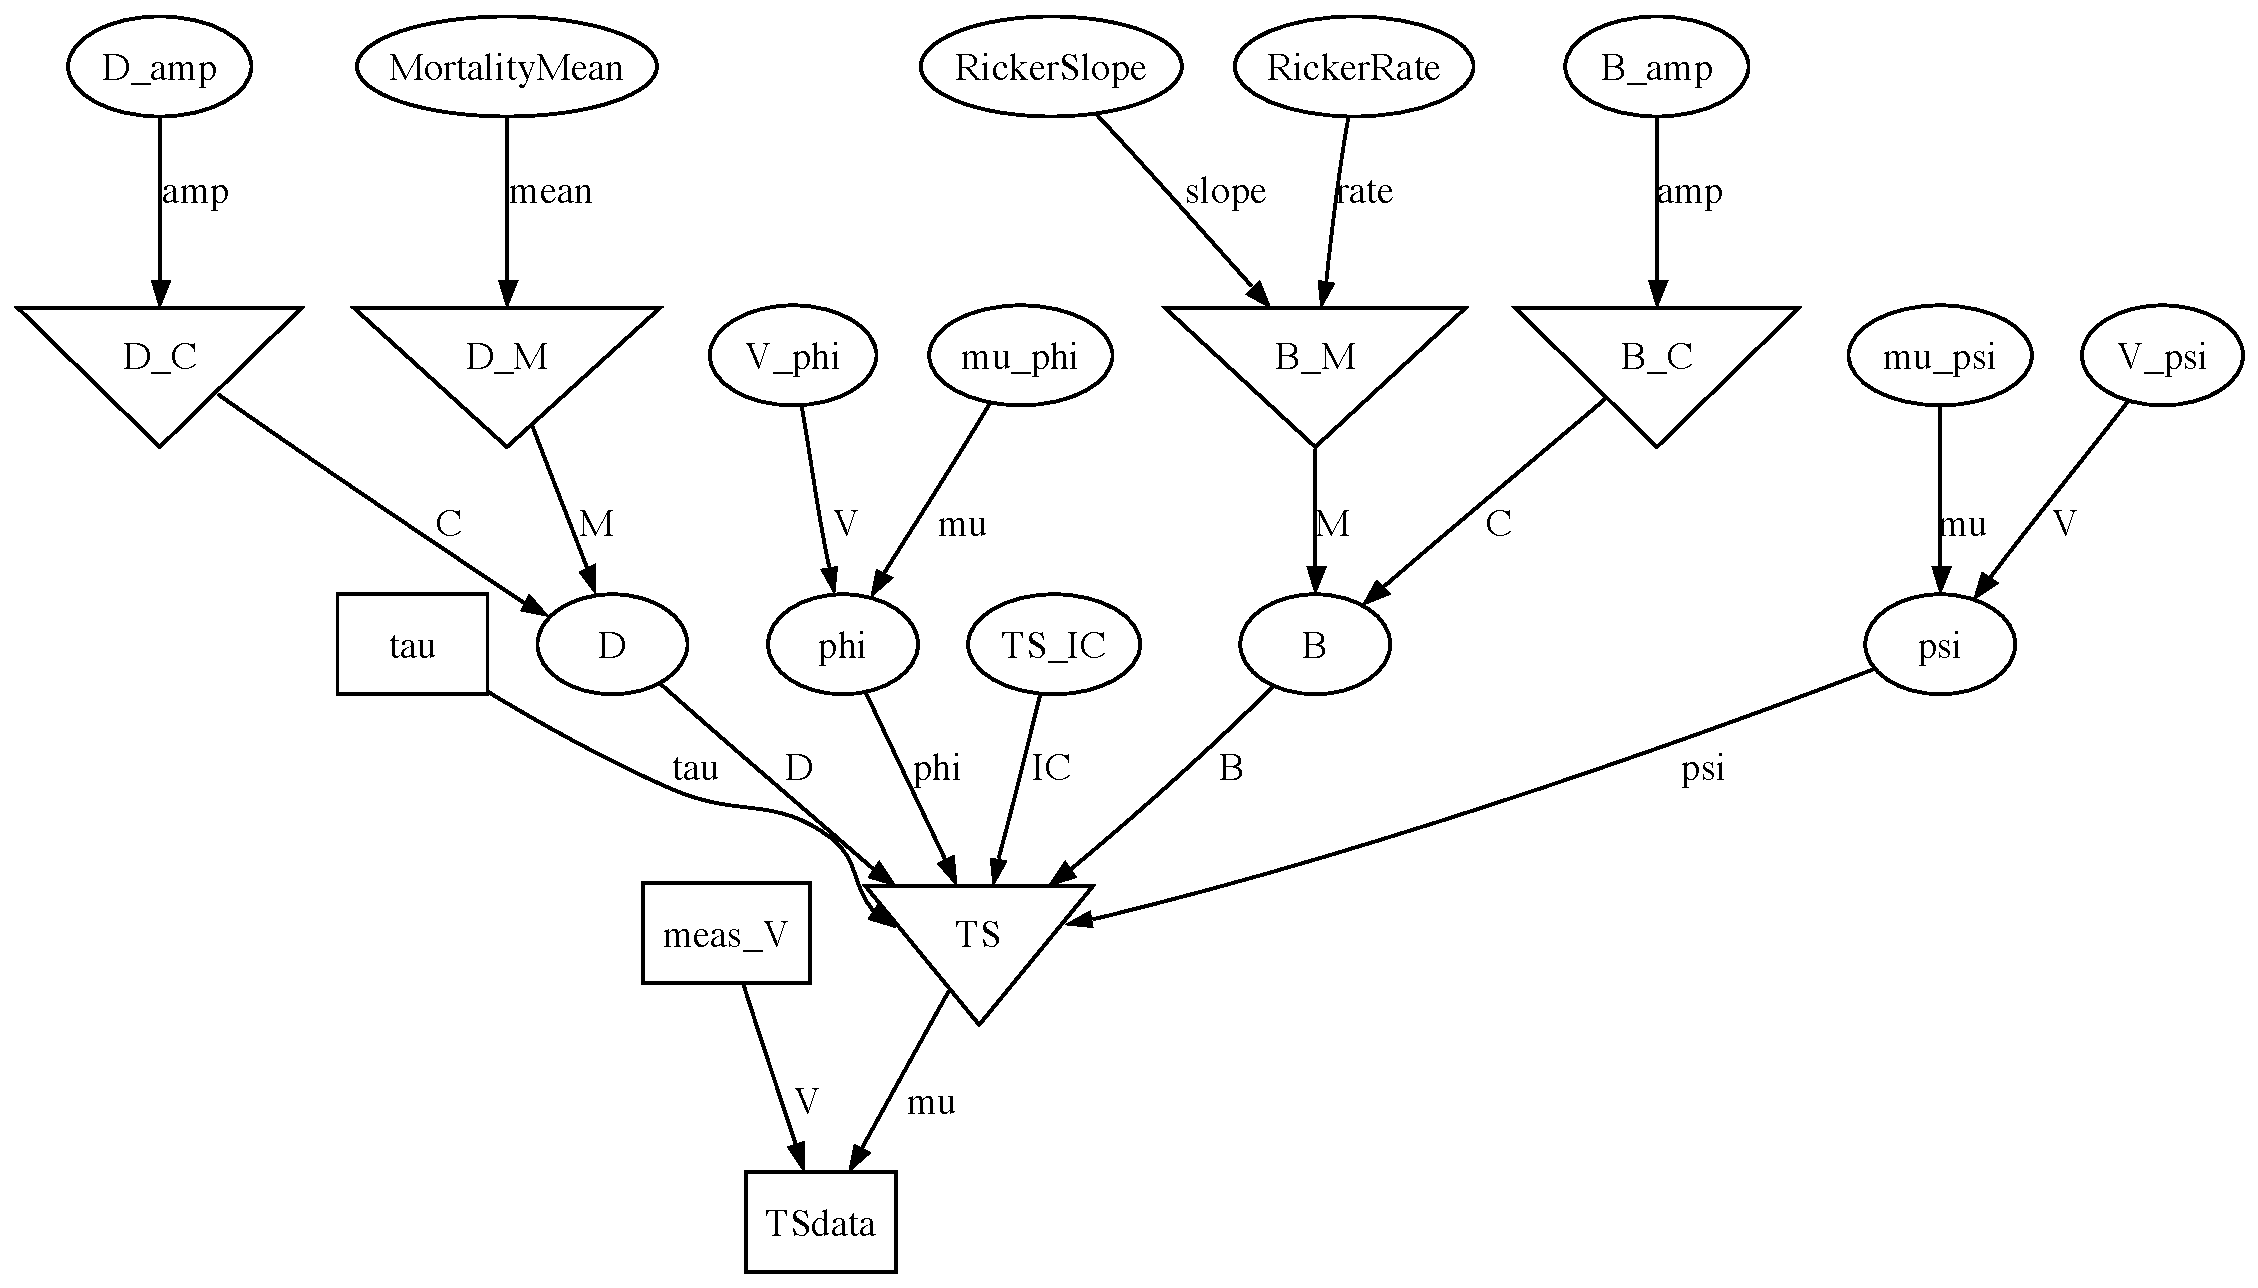
\epsfig{file=figs/ESSblowfly.pdf,width=15cm}
%     \caption{The model for Ellner, Seifu and Smith's \cite{ess} blowfly data.}
%     \label{fig:ESSblowflymodel}
% \end{figure}
%
% % \begin{figure}
% %     \centering
% %         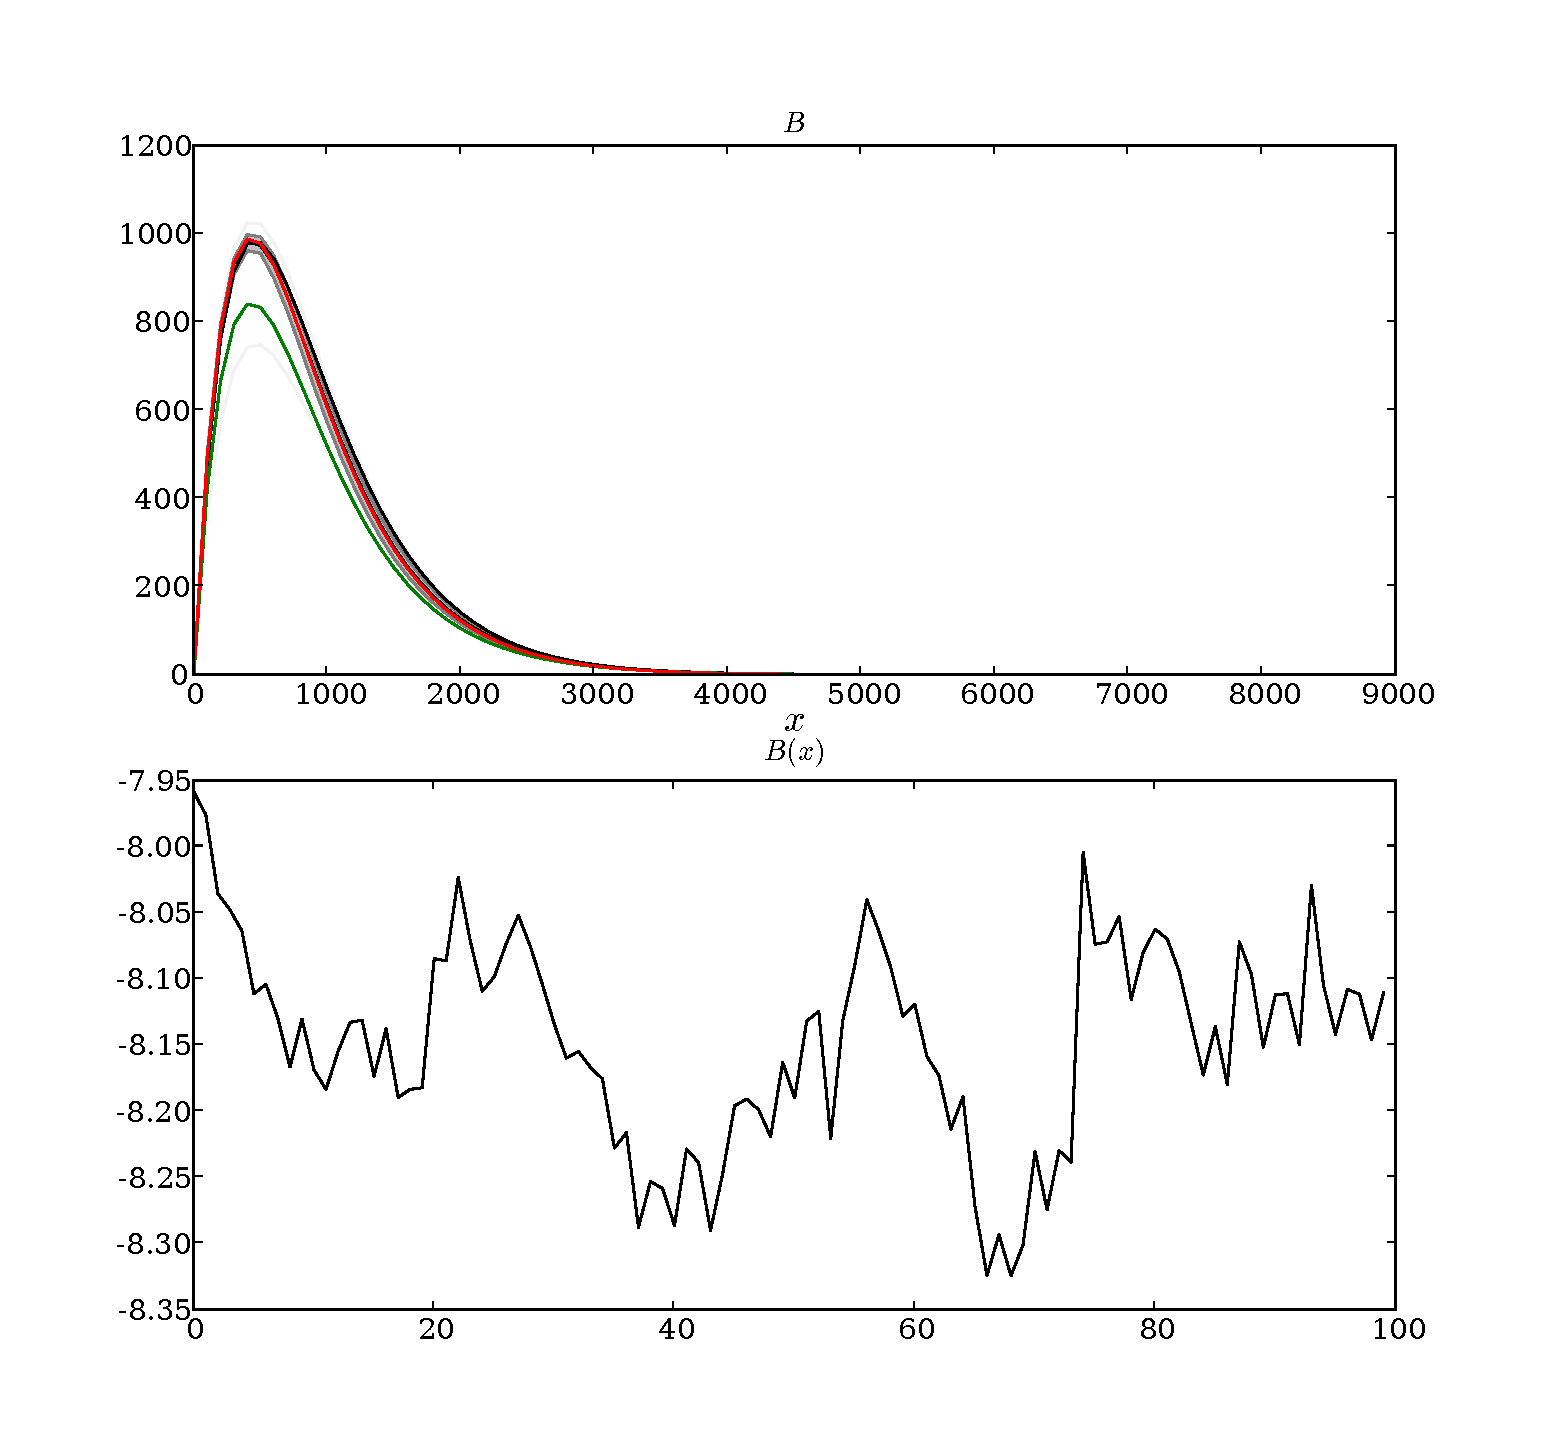
\epsfig{file=figs/ESSBPosterior.pdf,width=10cm}
% %         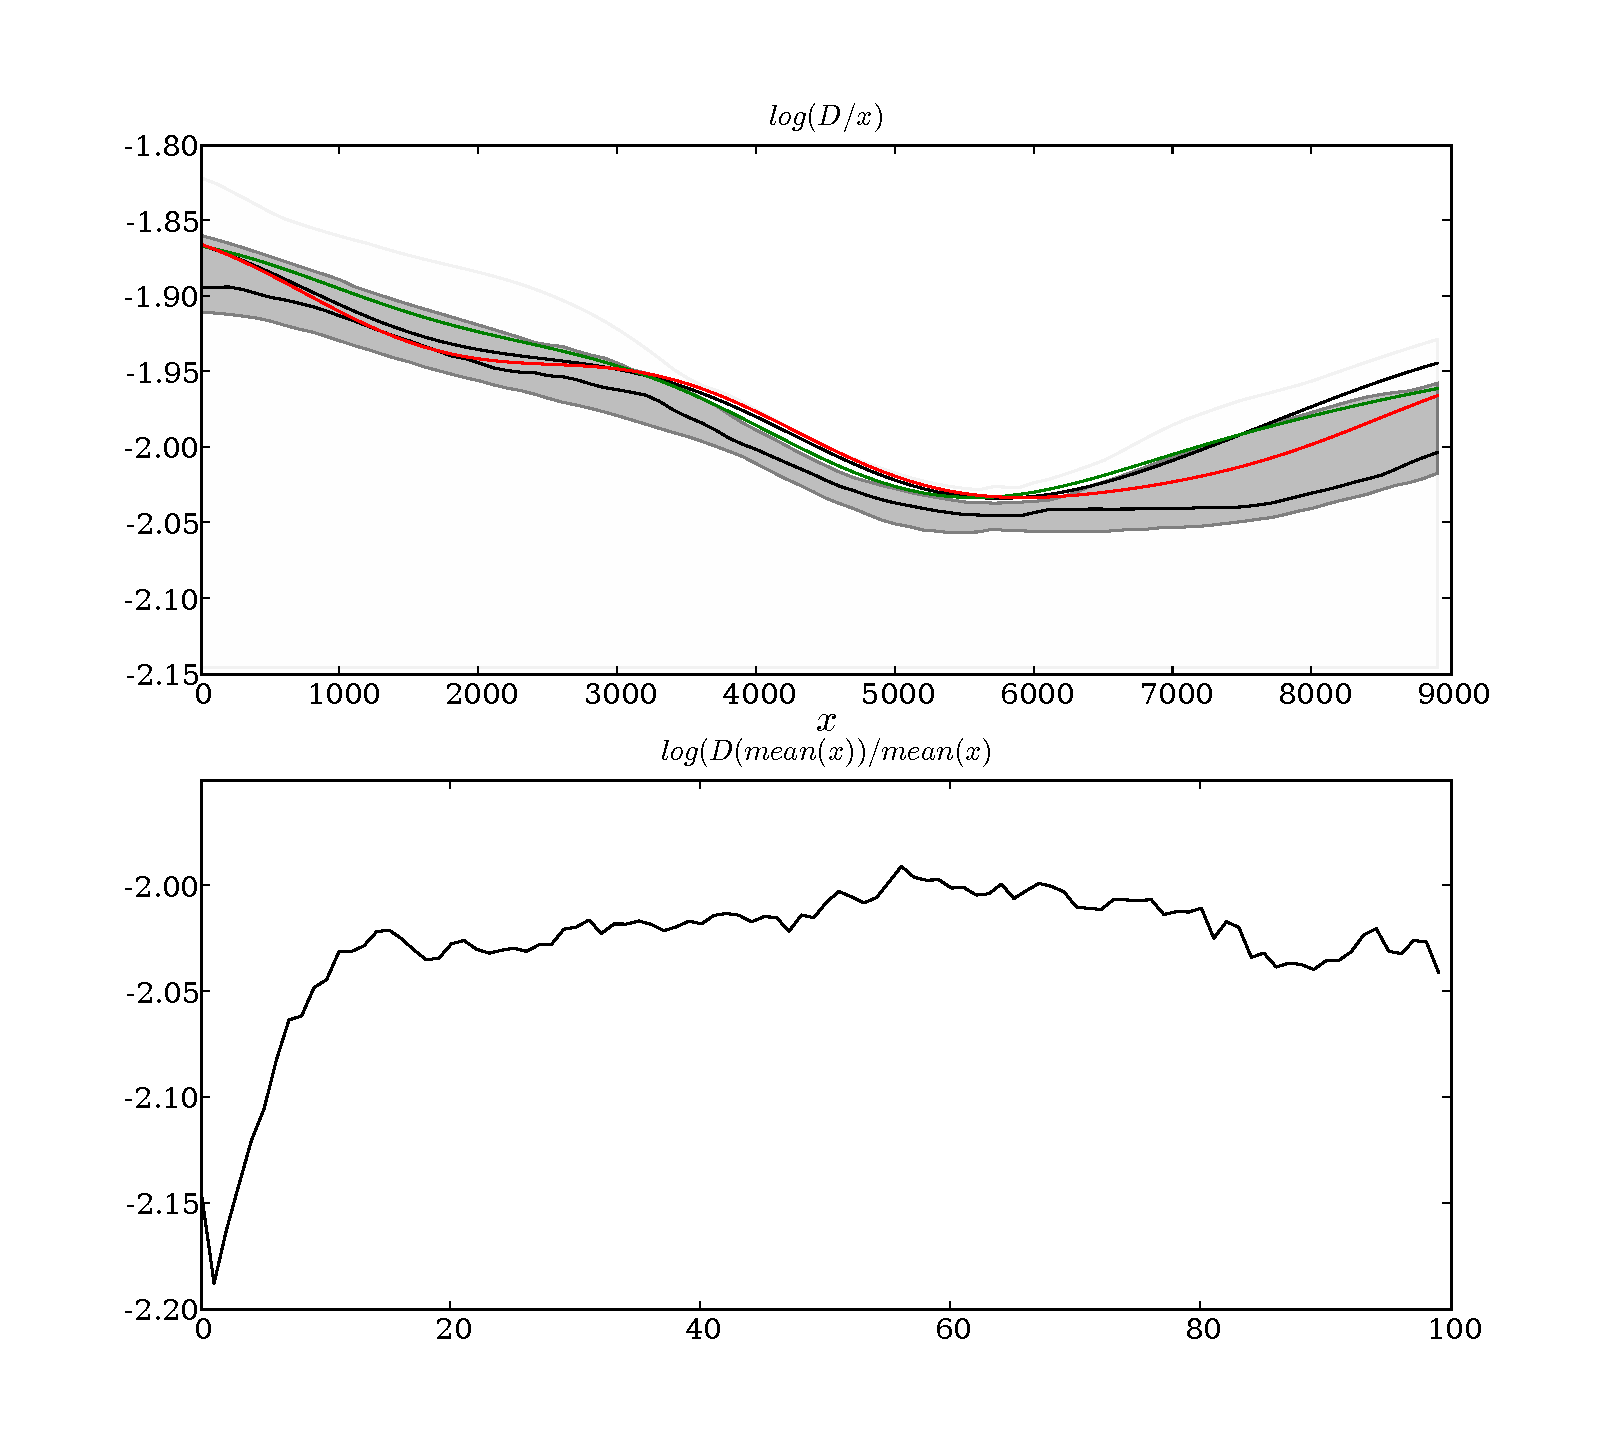
\epsfig{file=figs/ESSDPosterior.pdf,width=10cm}
% %     \caption{caption}
% %     \label{fig:ESSBD}
% % \end{figure}
% %
% % \begin{figure}
% %     \centering
% %         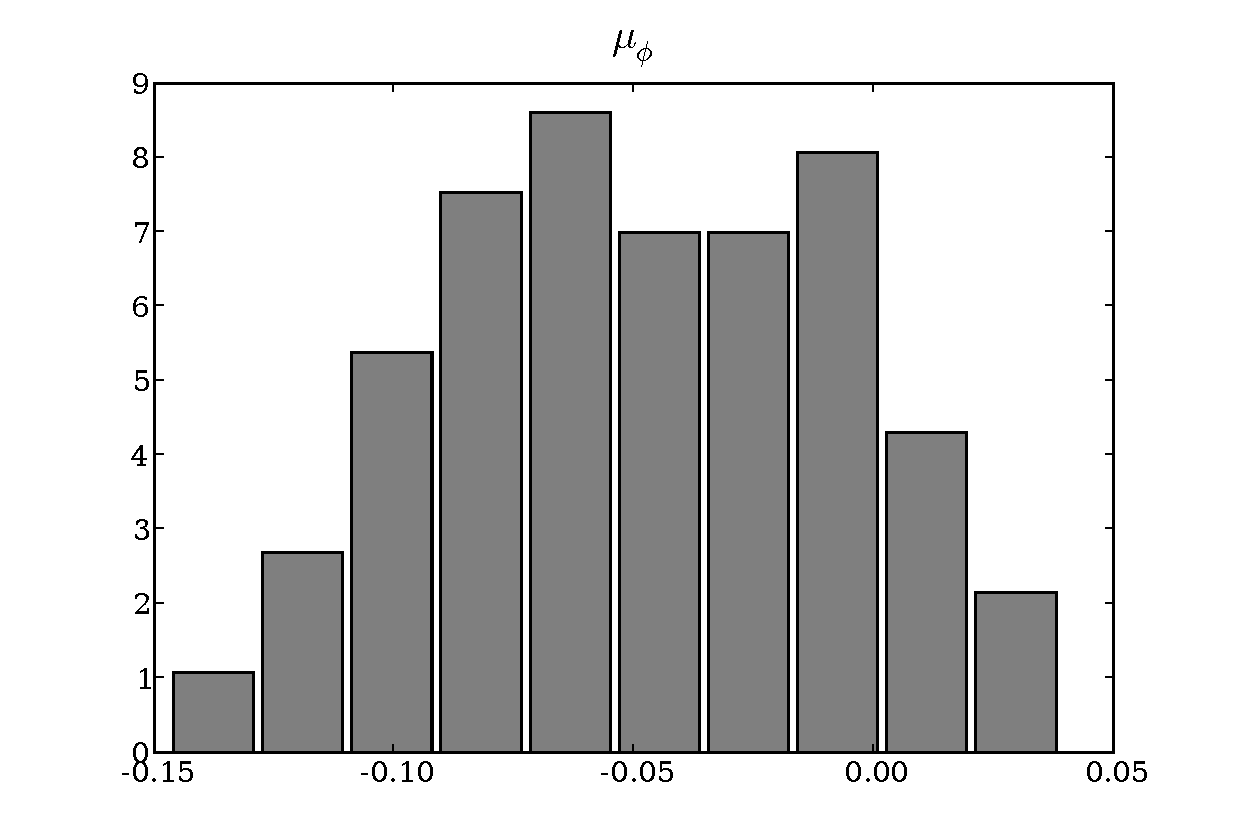
\epsfig{file=figs/ESSmuphiPosterior.pdf,width=7cm}
% %         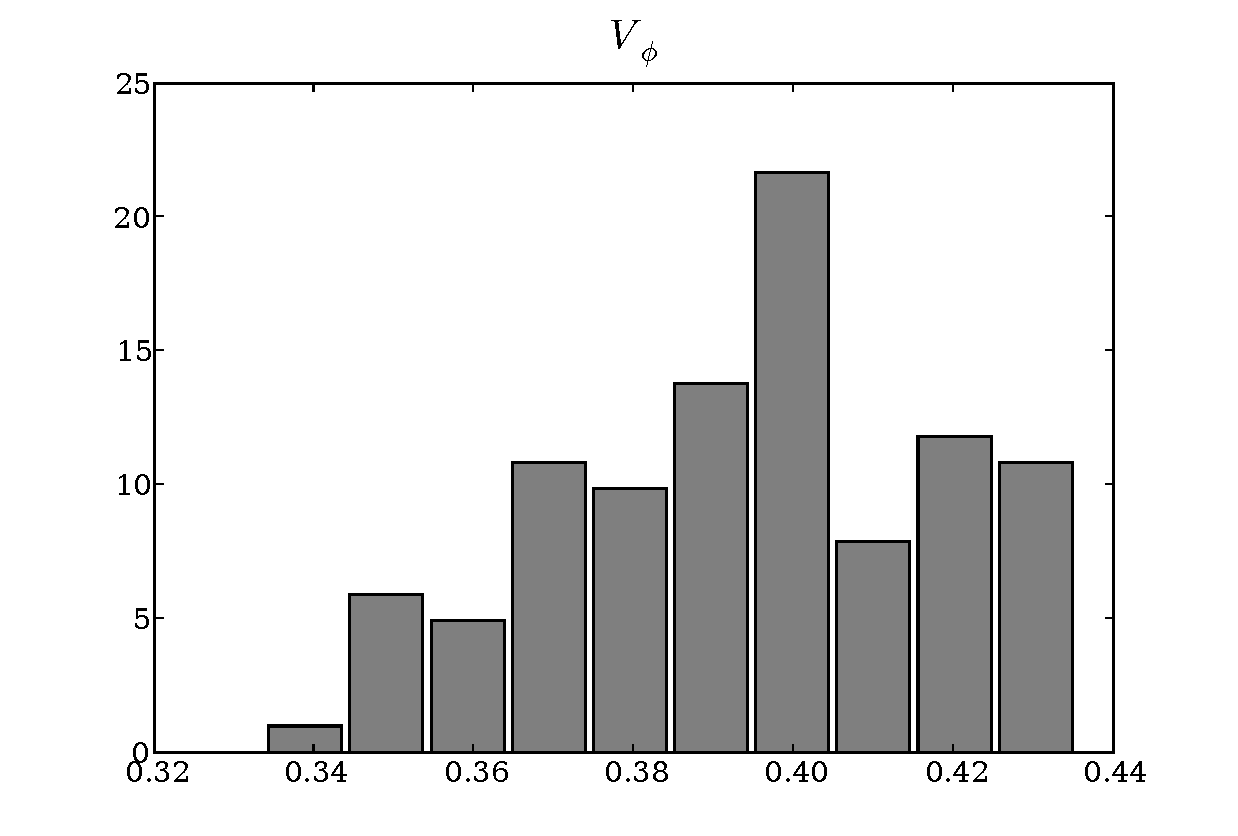
\epsfig{file=figs/ESSVphiPosterior.pdf,width=7cm}
% %         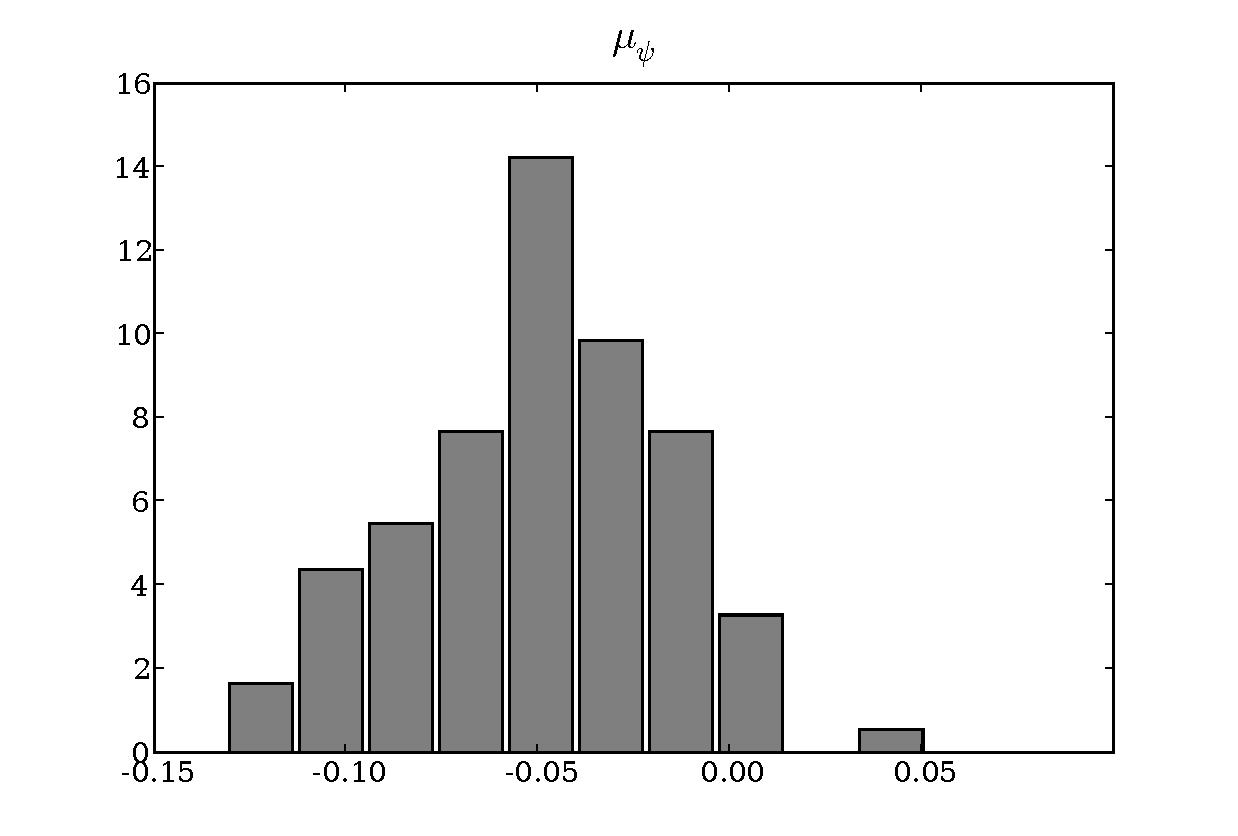
\epsfig{file=figs/ESSmupsiPosterior.pdf,width=7cm}
% %         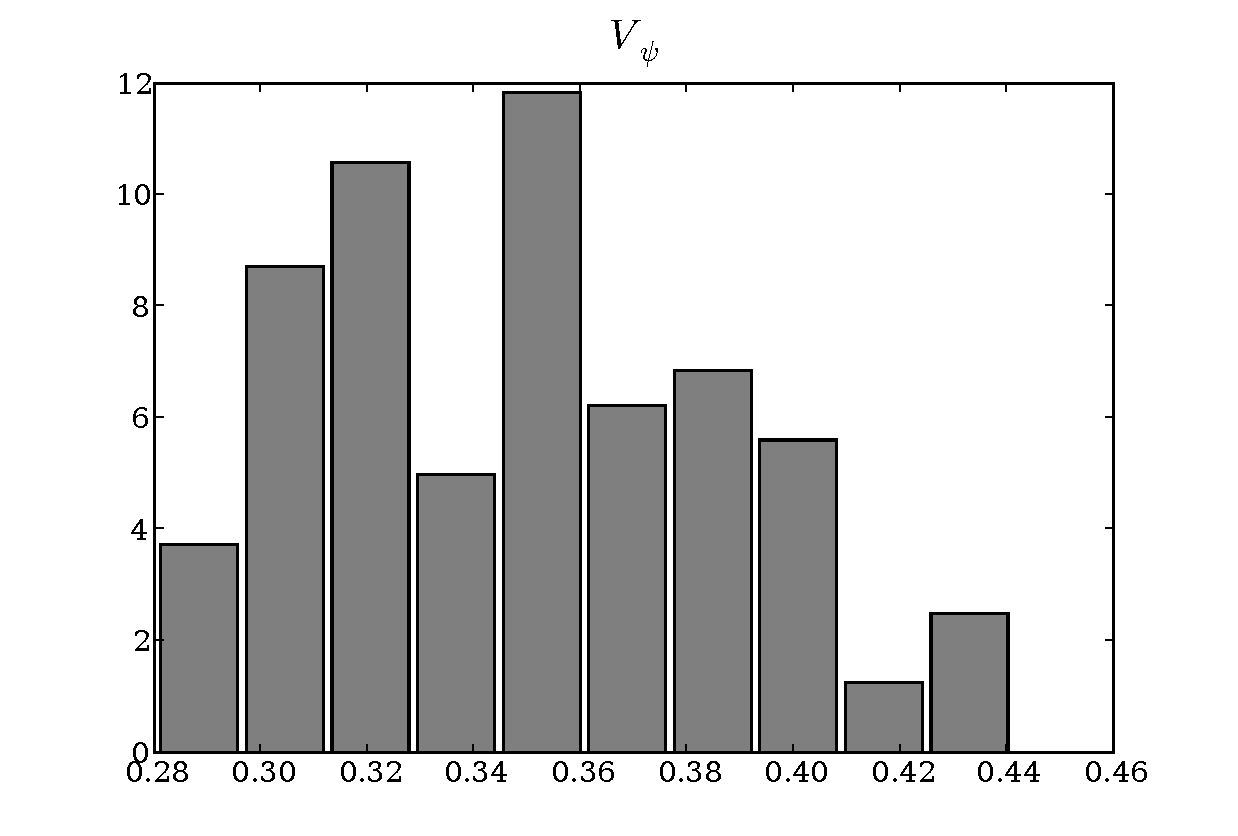
\epsfig{file=figs/ESSVpsiPosterior.pdf,width=7cm}
% %     \caption{caption}
% %     \label{fig:ESSphipsi}
% % \end{figure}
% %
% % \begin{figure}
% %     \centering
% %         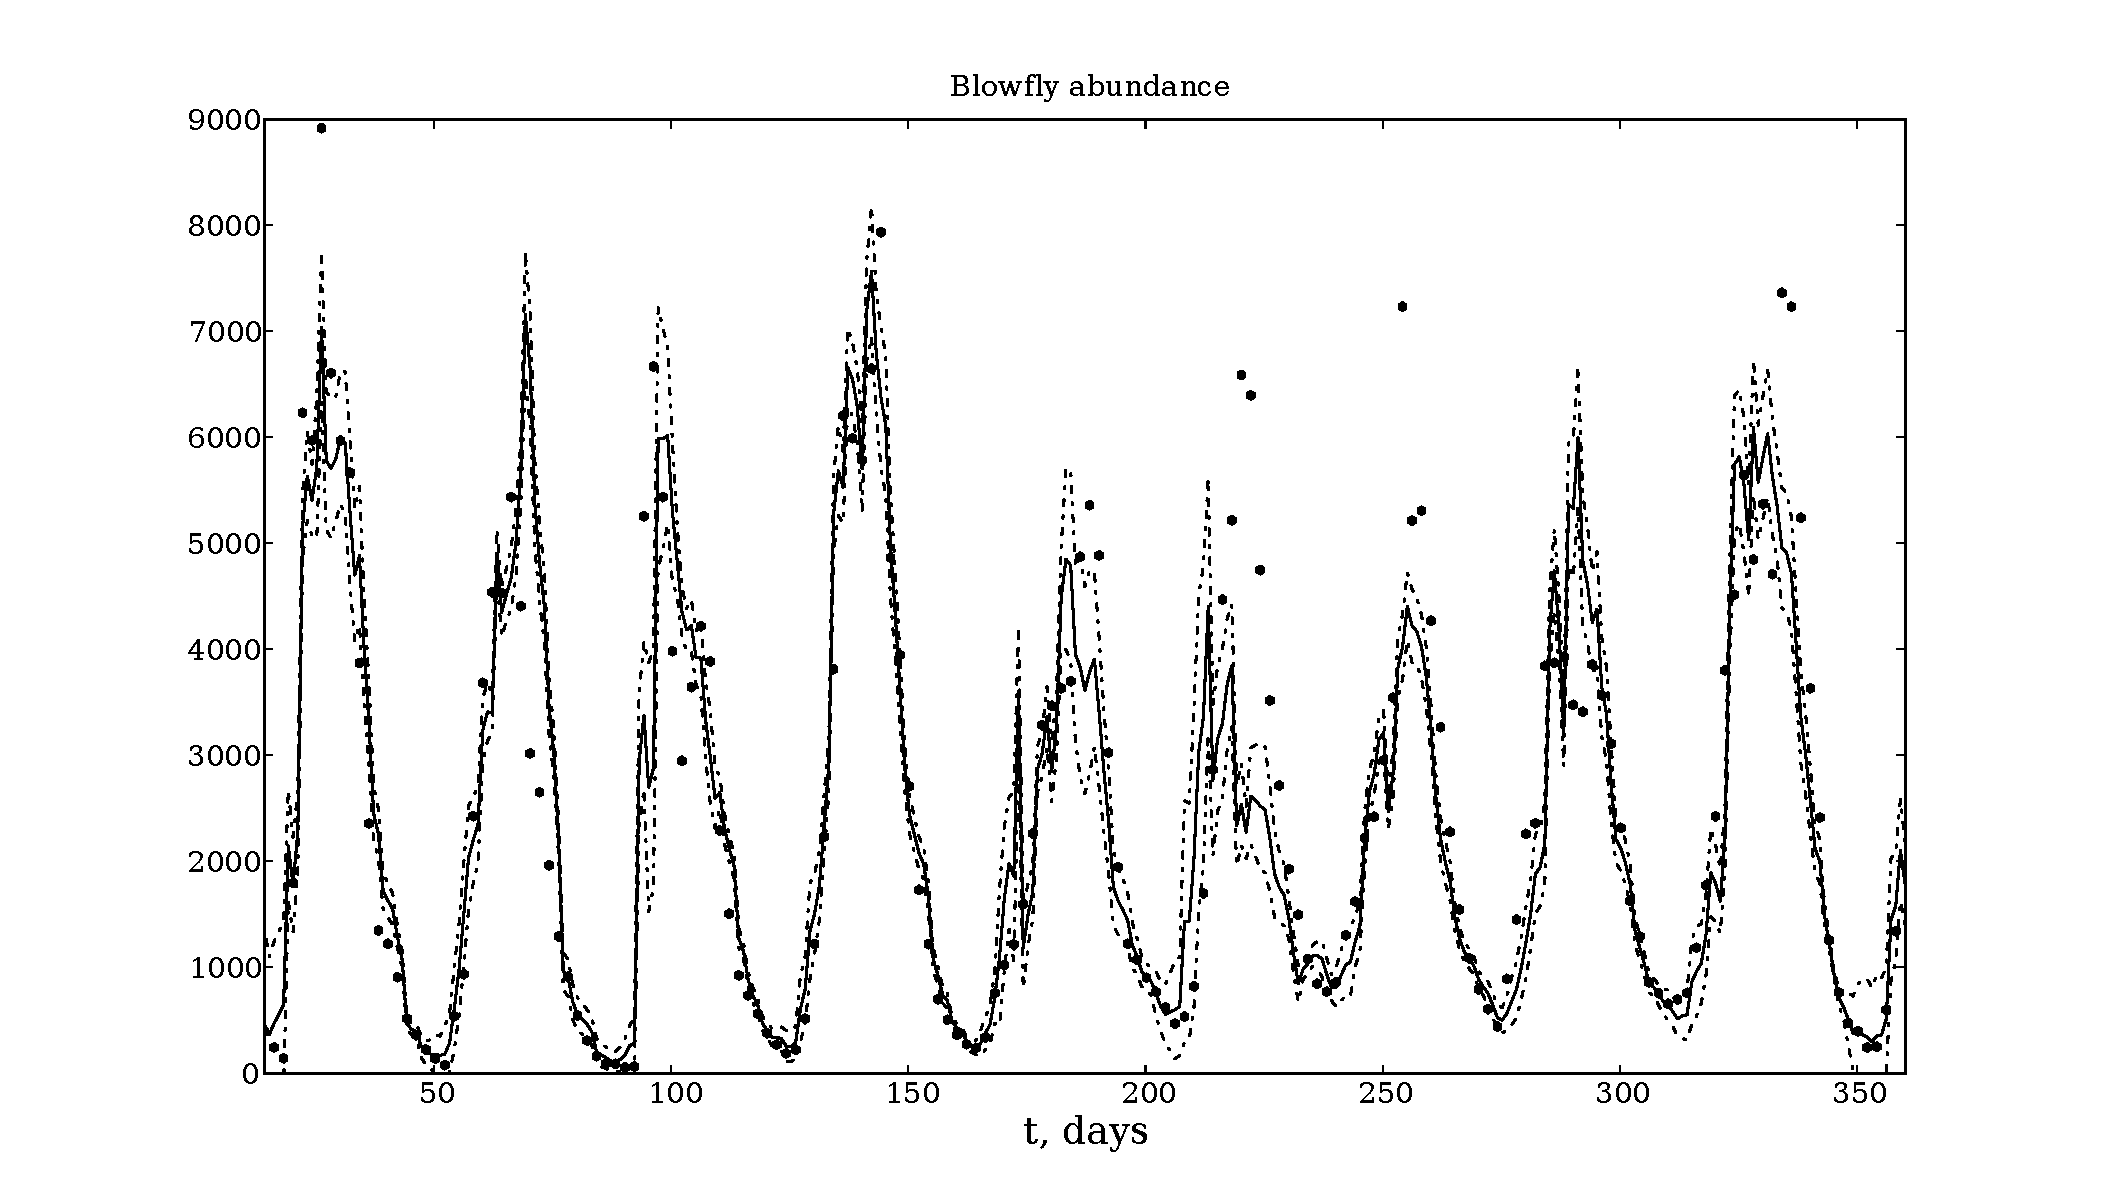
\epsfig{file=figs/ESSblowflyfit.pdf,width=15cm}
% %     \caption{caption}
% %     \label{fig:ESSfit}
% % \end{figure}
%
 


\section{Conclusion}

This package is built around the \code{Realization} object, which represents random mathematical functions as random \proglang{Python} functions. This is arguably the most natural and intuitive representation possible within the \proglang{Python} programming language, which itself is widely regarded as unusually human-friendly.

This package inherits the flexibility of PyMC, described in section \ref{sec:gp-sub}, in that the descendants of a Gaussian process can depend on it via any Python function. Because \pkg{PyMC} allows any \proglang{Python} function to be used to transform variables in probability models, \proglang{Python} (like all modern programming languages) allows functions to be passed to other functions as arguments, and \code{GP} objects are function-valued random variables, this package supports construction of an enormous variety of probability models that involve scalar-valued Gaussian processes. The Duffy negativity example in section \ref{sub:geostat} exhibits a probability model whose nonstandard likelihood function involves transformations of two Gaussian processes. In keeping with the extensible spirit of PyMC, the package accomodates user-specified covariance functions, and provides support for automatic combination of covariance functions and distance metrics.

Strenuous efforts at optimization have resulted in good performance for `standard' Gaussian process-based analyses such as Bayesian geostatistics. For example, \cite{map} recently used it to conduct a fully Bayesian MCMC analysis involving a very expensive covariance function evaluated at 4,291 input locations. The library of covariance functions provided by the package is implemented in Fortran, and can take advantage of SMP systems. The linear algebra functionality is provided by \code{NumPy}, which can be configured to make use of optimized, multithreaded BLAS and LAPACK \textbf{cite} implementations. 

However, there are use cases for which this package's flexible object model prevents it from achieving performance on par with hand-optimized algorithms. For example, the \code{mesh} attribute of \texttt{GPSubmodel} objects is fixed on creation, but in many reversible-jump MCMC applications (e.g. \cite{gramacy} and the toy example above) the set of input locations under consideration changes as the MCMC progresses. It would be possible to fit these models using \texttt{GPSubmodel}, but the acceptance rate would typically be much lower than that enjoyed by a true reversible-jump MCMC algorithm. It remains to be seen whether this and related performance problems can be overcome without either diluting the conceptual fidelity of the object model or incurring an unacceptable level of program complexity.

More tutorial material, as well as documentation of a few additional features and the incomplete Cholesky decomposition algorithms, can be found in the \href{http://pymc.googlecode.com/files/GPUserGuide.pdf}{package documentation}.

% \nocite{*}
% \bibliographystyle{plain}v
\bibliography{gp}

\end{document}
